\documentclass[a4paper,english,10pt]{article}\usepackage[]{graphicx}\usepackage[]{color}
%% maxwidth is the original width if it is less than linewidth
%% otherwise use linewidth (to make sure the graphics do not exceed the margin)
\makeatletter
\def\maxwidth{ %
  \ifdim\Gin@nat@width>\linewidth
    \linewidth
  \else
    \Gin@nat@width
  \fi
}
\makeatother

\definecolor{fgcolor}{rgb}{0.345, 0.345, 0.345}
\newcommand{\hlnum}[1]{\textcolor[rgb]{0.686,0.059,0.569}{#1}}%
\newcommand{\hlstr}[1]{\textcolor[rgb]{0.192,0.494,0.8}{#1}}%
\newcommand{\hlcom}[1]{\textcolor[rgb]{0.678,0.584,0.686}{\textit{#1}}}%
\newcommand{\hlopt}[1]{\textcolor[rgb]{0,0,0}{#1}}%
\newcommand{\hlstd}[1]{\textcolor[rgb]{0.345,0.345,0.345}{#1}}%
\newcommand{\hlkwa}[1]{\textcolor[rgb]{0.161,0.373,0.58}{\textbf{#1}}}%
\newcommand{\hlkwb}[1]{\textcolor[rgb]{0.69,0.353,0.396}{#1}}%
\newcommand{\hlkwc}[1]{\textcolor[rgb]{0.333,0.667,0.333}{#1}}%
\newcommand{\hlkwd}[1]{\textcolor[rgb]{0.737,0.353,0.396}{\textbf{#1}}}%

\usepackage{framed}
\makeatletter
\newenvironment{kframe}{%
 \def\at@end@of@kframe{}%
 \ifinner\ifhmode%
  \def\at@end@of@kframe{\end{minipage}}%
  \begin{minipage}{\columnwidth}%
 \fi\fi%
 \def\FrameCommand##1{\hskip\@totalleftmargin \hskip-\fboxsep
 \colorbox{shadecolor}{##1}\hskip-\fboxsep
     % There is no \\@totalrightmargin, so:
     \hskip-\linewidth \hskip-\@totalleftmargin \hskip\columnwidth}%
 \MakeFramed {\advance\hsize-\width
   \@totalleftmargin\z@ \linewidth\hsize
   \@setminipage}}%
 {\par\unskip\endMakeFramed%
 \at@end@of@kframe}
\makeatother

\definecolor{shadecolor}{rgb}{.97, .97, .97}
\definecolor{messagecolor}{rgb}{0, 0, 0}
\definecolor{warningcolor}{rgb}{1, 0, 1}
\definecolor{errorcolor}{rgb}{1, 0, 0}
\newenvironment{knitrout}{}{} % an empty environment to be redefined in TeX

\usepackage{alltt}
\usepackage{amsmath}
\usepackage{amssymb}
\usepackage{graphicx}
\usepackage{cite}
\usepackage{color} 
\usepackage{float}
\usepackage{longtable}
\usepackage[bottom]{footmisc}
\usepackage{url}
\usepackage{natbib}
\usepackage{authblk}
\usepackage[T1]{fontenc}
\usepackage[utf8x]{inputenc}
\usepackage{babel}
\usepackage{hyperref}
\usepackage{geometry}
\geometry{verbose,a4paper,tmargin=3cm,bmargin=2cm,lmargin=2cm,rmargin=3cm}
\setlength{\parskip}{\medskipamount}
\setlength{\parindent}{0pt}
\hypersetup{
    colorlinks=true,       % false: boxed links; true: colored links
    linkcolor=blue,        % color of internal links
    citecolor=red,         % color of links to bibliography
    filecolor=blue,        % color of file links
    urlcolor=blue          % color of external links
}

% Define some handy formatting
\newcommand{\code}[1]{{\texttt{#1}}}
\newcommand{\pkg}[1]{{\texttt{#1}}}
\newcommand{\class}[1]{{\textit{#1}}}
\newcommand{\R}{{\normalfont\textsf{R }}{}}
\newcommand{\args}[1]{{\texttt{#1}}}
\newcommand{\E}[1]{\text{E}\left[#1\right]}
\newcommand{\Var}[1]{\text{Var}\left[#1\right]}


%----------------------------------------------------------------------------------
\IfFileExists{upquote.sty}{\usepackage{upquote}}{}

\begin{document}
%\SweaveOpts{concordance=TRUE}

\title{Stock assessment and management advice with a4a methods \\ DRAFT}

\author[1]{Ernesto Jardim}
\author[1]{Colin Millar}
\author[1]{Finlay Scott}
\affil[1]{European Commission, Joint Research Centre, IPSC / Maritime Affairs Unit, 21027 Ispra (VA), Italy}
\affil[*]{Corresponding author \href{mailto:ernesto.jardim@jrc.ec.europa.eu}{ernesto.jardim@jrc.ec.europa.eu}}

\maketitle
\tableofcontents
\newpage

\section{Introduction}

\subsection{Background}

(This section is based on Jardim, et.al, 2014\footnote{Jardim,E., Millar,C.P., Mosqueira,I., Scott,F., Osio,G.C., Ferretti,M., Alzorriz,N., Orio,A. 2014. What if stock assessment is as simple as a linear model? The a4a initiative. ICES JMS. \url{http://icesjms.oxfordjournals.org/content/early/2014/04/03/icesjms.fsu050.abstract}
})

The volume and availability of data useful for fisheries stock assessment is continually increasing. Time series of ‘traditional’ sources of information, such as surveys and landings data are not only getting longer, but also cover an increasing number of species.

For example, in Europe the 2009 revision of the Data Collection Regulation (EU, 2008a) has changed the focus of fisheries sampling programmes away from providing data for individual assessment of ‘key’ stocks (i.e. those that are economically important) to documenting fishing trips, thereby shifting the perspective to a large coastal monitoring programme. The result has been that data on growth and reproduction of fish stocks are being collected for more than 300 stocks in waters where the European fleets operate.

Recognizing that the context above required new methodological developments, the European Commission Joint Research Centre (JRC) started its ‘Assessment for All’ Initiative (a4a), with the aim to develop, test, and distribute methods to assess a large numbers of stocks in an operational time frame, and to build the necessary capacity/expertise on stock assessment and advice provision. 

The long-term strategy of a4a is to increase the number of stock assessments by reducing the workload required to run each analysis and by bringing more scientists/analysts into fisheries management advice. The first is achieved by developing a working framework with the methods required to run all the analysis a stock assessment needs, as well as developing methods to deal with recognized bottlenecks, \emph{e.g.} model averaging to deal with model selection. Such an approach should make the model exploration and selection processes easier, as well as decreasing the burden of moving between software platforms. The second can be achieved by making the analysis more intuitive, thereby attracting more experts to join stock assessment teams.

To achieve these objectives, the Initiative identified a series of tasks, which were or are being carried out, namely:
\begin{itemize}
	\item define a moderate data stock;
	\item develop a stock assessment framework;
	\item develop a forecasting algorithm based on MSE;
	\item organize training courses for marine scientists.
\end{itemize}

\subsubsection{The moderate data stock}

The moderate data stock definition was an important step in the Initiative's development. It clearly focused the initiative on stocks with some information, moving away from the data-poor stocks, but without moving into data eager methodologies. It was recognized that there's a lot of research on both extremes of the data availability spectrum, but the middle 'region' is most of the times left behind.

The 'moderate data stock', which constitutes the entry level of our analysis, has at least the following datasets, which can be assembled in different ways, using distinct methods.
 
\begin{itemize}
	\item in relation to exploitation:
	\begin{itemize}
		\item nominal effort (optional, needed in case CPUE indices are to be derived);
		\item volume of catches, which may be split in landings and discards, or not;
		\item length frequencies of the catches, landings or discards;
	\end{itemize}
	\item in relation to biology:
	\begin{itemize}
		\item knife edge maturity ogive;
		\item indication of growth model and parameters;
		\item length-weight relationship;
	\end{itemize}
	\item in relation to abundance:
	\begin{itemize}
		\item index of abundance.
	\end{itemize}	
\end{itemize}

\subsubsection{The stock assessment framework}

The stock assessment model framework is a non-Linear catch-at-age model implemented in R/FLR/ADMB that can be applied rapidly to a wide range of situations with low parametrization requirements. Later we'll come back to these characteristics and it's application.

\subsubsection{MSE}

Regarding the MSE, it's seen as a sophisticated forecasting algorithm that takes into account structural uncertainty about stock dynamics (growth, recruitment, maturity) and on exploitation by commercial fleets (selectivity), embedding the framework of decision making. 

\subsubsection{Training}

During the last 2 years JRC organized 4 courses of introduction to R and FLR: Varese, January 2012; Varese, ??? ...

In 2013 a short course about a4a methods was organized in Lisbon, the first full course on FLR and a4a methods was organized in CEFAS, March 2014 and another one is planned for August 2014.

These courses are open to all participants and don't have an attendance fee.

\subsection{The a4a approach to stock assessment and management advice}

The approach presented here is split in 4 steps: (i) converting length data to age data using a growth model, (ii) modelling natural mortality, (iii) assessing the stock, and (iv) MSE\footnote{Under development, to be released with version 2.0, scheduled for the fourth quarter of 2014}.

These steps may be followed in sequence or independently, depending on the user's preferences. All that is needed is to use the objects provided by the previous step and provide the objects required by the next, so that data flows between steps smoothly. One can make the analogy with a lego build, where for each layer the builder may use the pieces provided by a particular boxset, or make use of pieces from other boxsets. Figure \ref{fig:inout} shows the process including the class of the objects that carry the data (in black).

\begin{figure}[h]
\centering
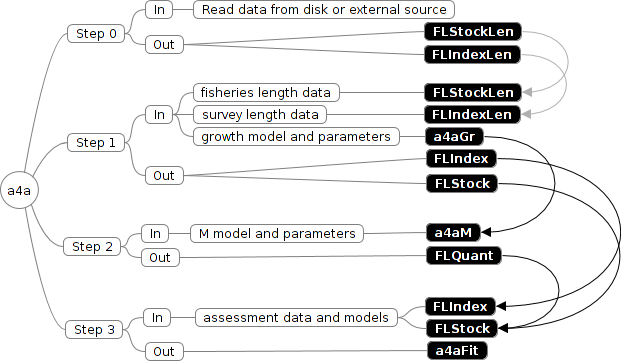
\includegraphics[width=\textwidth]{./inout}
\caption{In/out process of the a4a approach. The boxes in black represent the classes of the objects that carry the information for each step and out of each step.}
\label{fig:inout}
\end{figure}

Analysis related with projections and biological reference points are dealt by the FLR packages FLash and FLBRP. As such the Initiative does not provide specific methods for these analysis.

Steps 1 and 2 are simulation based, there's no fitting of growth models or natural mortality models. The rationale is to provide tools that allow the uncertainty associated with these processes to be carried on into the stock assessment. This approach allows the users to pick up the required information from other sources of information, like papers, PhDs, Fishbase, other stocks, etc. Baring in mind that the entry level stock may not have hard information on the processes of growth or natural mortality, but generic information about life history invariants can be used. For example, Nokome Bentley is developing an R package that uses bayesian networks to estimate empirical distributions for these parameters from Fishbase.

\subsection{Loading libraries, data and defining some useful functions}

\begin{knitrout}
\definecolor{shadecolor}{rgb}{0.969, 0.969, 0.969}\color{fgcolor}\begin{kframe}
\begin{alltt}
\hlkwd{library}\hlstd{(FLa4a)}
\hlkwd{library}\hlstd{(XML)}
\hlkwd{library}\hlstd{(reshape2)}
\hlkwd{library}\hlstd{(diagram)}
\hlkwd{data}\hlstd{(ple4)}
\hlkwd{data}\hlstd{(ple4.indices)}
\end{alltt}
\end{kframe}
\end{knitrout}





\begin{knitrout}
\definecolor{shadecolor}{rgb}{1, 1, 1}\color{fgcolor}\begin{kframe}
\begin{verbatim}
# functions for transforming the data

# quant 2 quant
qt2qt <- function(object, id = 5, split = "-") {
    qt <- object[, id]
    levels(qt) <- unlist(lapply(strsplit(levels(qt), split = split), "[[", 2))
    as.numeric(as.character(qt))
}

# check import and massage
cim <- function(object, n, wt, hrv = "missing") {
    v <- object[sample(1:nrow(object), 1), ]
    c1 <- c(n[as.character(v$V5), as.character(v$V1), 1, as.character(v$V2)] == 
        v$V6)
    c2 <- c(wt[as.character(v$V5), as.character(v$V1), 1, as.character(v$V2)] == 
        v$V7)
    if (missing(hrv)) {
        c1 + c2 == 2
    } else {
        c3 <- c(hrv[as.character(v$V5), as.character(v$V1), 1, as.character(v$V2)] == 
            v$V8)
        c1 + c2 + c3 == 3
    }
}

# and a plot for later
plotS4 <- function(object, linktext = "typeof", main = "S4 class", ...) {
    args <- list(...)
    obj <- getClass(as.character(object))
    df0 <- data.frame(names(obj@slots), unlist(lapply(obj@slots, "[[", 1)))
    nms <- c(t(df0))
    nslts <- length(nms)/2
    M <- matrix(nrow = length(nms), ncol = length(nms), byrow = TRUE, data = 0)
    for (i in 1:nslts) {
        M[i * 2, i * 2 - 1] <- linktext
    }
    args$A = M
    args$pos = rep(2, length(nms)/2)
    args$name = nms
    args$main = main
    do.call("plotmat", args)
}
\end{verbatim}
\end{kframe}
\end{knitrout}


\section{Reading files and building FLR objects}

For this document we'll use the plaice in ICES area IV dataset, provided by FLR, and a length-based simulated dataset based on red fish, using Gadget (http://www.hafro.is/gadget), provided by Daniel Howell (Institute of Marine Research, Norway).

In this section we read in the Gadget data files, and transform them into FLR objects.

First we read in the files as data frames and recode some variables.

\begin{knitrout}
\definecolor{shadecolor}{rgb}{1, 1, 1}\color{fgcolor}\begin{kframe}
\begin{verbatim}
# catch
cth.orig <- read.table("data/catch.len", skip = 5)

# stock
stk.orig <- read.table("data/red.len", skip = 4)

# surveys
idx.orig <- read.table("data/survey.len", skip = 5)
idxJmp.orig <- read.table("data/jump.survey.len", skip = 5)
idxTrd.orig <- read.table("data/tend.survey.len", skip = 5)

# Recode the length categories into something usable

# catch
cth.orig[, 5] <- qt2qt(cth.orig)

# stock
stk.orig[, 5] <- qt2qt(stk.orig)

# surveys
idx.orig[, 5] <- qt2qt(idx.orig)
idxJmp.orig[, 5] <- qt2qt(idxJmp.orig)
idxTrd.orig[, 5] <- qt2qt(idxTrd.orig)
\end{verbatim}
\end{kframe}
\end{knitrout}


Then we reshape the data frames into six dimensional arrays using cast from package 'reshape2'.

\begin{knitrout}
\definecolor{shadecolor}{rgb}{1, 1, 1}\color{fgcolor}\begin{kframe}
\begin{verbatim}
# catch
cth.n <- acast(V5 ~ V1 ~ 1 ~ V2 ~ 1 ~ 1, value.var = "V6", data = cth.orig)
cth.wt <- acast(V5 ~ V1 ~ 1 ~ V2 ~ 1 ~ 1, value.var = "V7", data = cth.orig)
hrv <- acast(V5 ~ V1 ~ 1 ~ V2 ~ 1 ~ 1, value.var = "V8", data = cth.orig)

# stock
stk.n <- acast(V5 ~ V1 ~ 1 ~ V2 ~ 1 ~ 1, value.var = "V6", data = stk.orig)
stk.wt <- acast(V5 ~ V1 ~ 1 ~ V2 ~ 1 ~ 1, value.var = "V7", data = stk.orig)

# surveys
idx.n <- acast(V5 ~ V1 ~ 1 ~ V2 ~ 1 ~ 1, value.var = "V6", data = idx.orig)
idx.wt <- acast(V5 ~ V1 ~ 1 ~ V2 ~ 1 ~ 1, value.var = "V7", data = idx.orig)
idx.hrv <- acast(V5 ~ V1 ~ 1 ~ V2 ~ 1 ~ 1, value.var = "V8", data = idx.orig)
idxJmp.n <- acast(V5 ~ V1 ~ 1 ~ V2 ~ 1 ~ 1, value.var = "V6", data = idxJmp.orig)
idxJmp.wt <- acast(V5 ~ V1 ~ 1 ~ V2 ~ 1 ~ 1, value.var = "V7", data = idxJmp.orig)
idxJmp.hrv <- acast(V5 ~ V1 ~ 1 ~ V2 ~ 1 ~ 1, value.var = "V8", data = idxJmp.orig)
idxTrd.n <- acast(V5 ~ V1 ~ 1 ~ V2 ~ 1 ~ 1, value.var = "V6", data = idxTrd.orig)
idxTrd.wt <- acast(V5 ~ V1 ~ 1 ~ V2 ~ 1 ~ 1, value.var = "V7", data = idxTrd.orig)
idxTrd.hrv <- acast(V5 ~ V1 ~ 1 ~ V2 ~ 1 ~ 1, value.var = "V8", data = idxTrd.orig)
\end{verbatim}
\end{kframe}
\end{knitrout}


We take the arrays and make \class{FLQuant} objects from them.

\begin{knitrout}
\definecolor{shadecolor}{rgb}{1, 1, 1}\color{fgcolor}\begin{kframe}
\begin{verbatim}
# catch
dnms <- dimnames(cth.n)
names(dnms) <- names(dimnames(FLQuant()))
names(dnms)[1] <- "len"
cth.n <- FLQuant(cth.n, dimnames = dnms)
cth.wt <- FLQuant(cth.wt, dimnames = dnms)
hrv <- FLQuant(hrv, dimnames = dnms)
units(hrv) <- "f"

# stock
dnms <- dimnames(stk.n)
names(dnms) <- names(dimnames(FLQuant()))
names(dnms)[1] <- "len"
stk.n <- FLQuant(stk.n, dimnames = dnms)
stk.wt <- FLQuant(stk.wt, dimnames = dnms)

# surveys
dnms <- dimnames(idx.n)
names(dnms) <- names(dimnames(FLQuant()))
names(dnms)[1] <- "len"
idx.n <- FLQuant(idx.n, dimnames = dnms)
idx.wt <- FLQuant(idx.wt, dimnames = dnms)
idx.hrv <- FLQuant(idx.hrv, dimnames = dnms)

dnms <- dimnames(idxJmp.n)
names(dnms) <- names(dimnames(FLQuant()))
names(dnms)[1] <- "len"
idxJmp.n <- FLQuant(idxJmp.n, dimnames = dnms)
idxJmp.wt <- FLQuant(idxJmp.wt, dimnames = dnms)
idxJmp.hrv <- FLQuant(idxJmp.hrv, dimnames = dnms)

dnms <- dimnames(idxTrd.n)
names(dnms) <- names(dimnames(FLQuant()))
names(dnms)[1] <- "len"
idxTrd.n <- FLQuant(idxTrd.n, dimnames = dnms)
idxTrd.wt <- FLQuant(idxTrd.wt, dimnames = dnms)
idxTrd.hrv <- FLQuant(idxTrd.hrv, dimnames = dnms)
\end{verbatim}
\end{kframe}
\end{knitrout}


Some sanity checks to check that the resulting objects have matching dimensions.

\begin{knitrout}
\definecolor{shadecolor}{rgb}{1, 1, 1}\color{fgcolor}\begin{kframe}
\begin{verbatim}
# catch
cim(cth.orig, cth.n, cth.wt, hrv)
## [1] TRUE

# stock
cim(stk.orig, stk.n, stk.wt)
## [1] TRUE

# surveys
cim(idx.orig, idx.n, idx.wt, idx.hrv)
## [1] TRUE
cim(idxJmp.orig, idxJmp.n, idxJmp.wt, idxJmp.hrv)
## [1] TRUE
cim(idxTrd.orig, idxTrd.n, idxTrd.wt, idxTrd.hrv)
## [1] TRUE
\end{verbatim}
\end{kframe}
\end{knitrout}


%#------------------------------------------------------------------------------
%# contents
%#------------------------------------------------------------------------------

%# length-weight relationship is a bit odd ...
%xyplot(data~len|year, groups=season, data=cth.wt/cth.n, type="l")

%# length-weight relationship is a bit odd ...
%xyplot(data~len|year, groups=season, data=stk.wt, type="l")

Finally, we make FLR objects from the data.

\begin{knitrout}
\definecolor{shadecolor}{rgb}{1, 1, 1}\color{fgcolor}\begin{kframe}
\begin{verbatim}
# stock
rfLen.stk <- FLStockLen(stock.n = stk.n, stock.wt = stk.wt, stock = quantSums(stk.wt * 
    stk.n), catch.n = cth.n, catch.wt = cth.wt/cth.n, catch = quantSums(cth.wt), 
    harvest = hrv)
m(rfLen.stk)[] <- 0.05
mat(rfLen.stk)[] <- m.spwn(rfLen.stk)[] <- harvest.spwn(rfLen.stk)[] <- 0
mat(rfLen.stk)[38:59, , , 3:4] <- 1

# surveys
rfTrawl.idx <- FLIndex(index = idx.n, catch.n = idx.n, catch.wt = idx.wt, sel.pattern = idx.hrv)
effort(rfTrawl.idx)[] <- 100

rfTrawlJmp.idx <- FLIndex(index = idxJmp.n, catch.n = idxJmp.n, catch.wt = idxJmp.wt, 
    sel.pattern = idxJmp.hrv)
effort(rfTrawlJmp.idx)[] <- 100

rfTrawlTrd.idx <- FLIndex(index = idxTrd.n, catch.n = idxTrd.n, catch.wt = idxTrd.wt, 
    sel.pattern = idxTrd.hrv)
effort(rfTrawlTrd.idx)[] <- 100
\end{verbatim}
\end{kframe}
\end{knitrout}


\pagebreak
\section{Converting length data to age}

The stock assessment framework is based on age dynamics. To use length information it must be pre-processed before used for assessment. The rationale is that the pre-processing should give the analyst the flexibility to use a range of sources of information, \emph{e.g.} literature or online databases, to grab information about the species growth and the uncertainty about the model parameters.

Within the a4a framework this is handled using the \class{a4aGr} class. In this section we introduce the \class{a4aGr} class and look at the variety of ways that parameter uncertainty can be included.

\subsection{a4aGr - The growth class}

The convertion of length data to age is performed through the use of a growth model. The implementation is done through the \class{a4aGr} class.

\begin{knitrout}
\definecolor{shadecolor}{rgb}{1, 1, 1}\color{fgcolor}\begin{kframe}
\begin{verbatim}
showClass("a4aGr")
## Class "a4aGr" [package "FLa4a"]
## 
## Slots:
##                                                                   
## Name:      grMod  grInvMod    params      vcov     distr      name
## Class:   formula   formula     FLPar     array character character
##                           
## Name:       desc     range
## Class: character   numeric
## 
## Extends: "FLComp"
\end{verbatim}
\end{kframe}
\end{knitrout}


A simple construction of \class{a4aGr} objects requires the model and parameters to be provided.
Check the help file for more information.

Here we show an example using the von Bertalanffy growth model. To create the \class{a4aGr} object it's necessary to pass the model equation ($length \sim time$), the inverse model equation ($time \sim length$) and the parameters. Any growth model can be used as long as it's possible to write the equation in the form explained.

\begin{knitrout}
\definecolor{shadecolor}{rgb}{1, 1, 1}\color{fgcolor}\begin{kframe}
\begin{verbatim}
vbObj <- a4aGr(grMod = ~linf * (1 - exp(-k * (t - t0))), grInvMod = ~t0 - 1/k * 
    log(1 - len/linf), params = FLPar(linf = 58.5, k = 0.086, t0 = 0.001, units = c("cm", 
    "ano-1", "ano")))

# Check the model and its inverse
lc = 20
predict(vbObj, len = lc)
##    iter
##         1
##   1 4.866
predict(vbObj, t = predict(vbObj, len = lc)) == lc
##    iter
##        1
##   1 TRUE
\end{verbatim}
\end{kframe}
\end{knitrout}


The predict method allows the transformation between age and lengths.

\begin{knitrout}
\definecolor{shadecolor}{rgb}{1, 1, 1}\color{fgcolor}\begin{kframe}
\begin{verbatim}
predict(vbObj, len = 5:10 + 0.5)
##    iter
##         1
##   1 1.149
##   2 1.371
##   3 1.596
##   4 1.827
##   5 2.062
##   6 2.301
predict(vbObj, t = 5:10 + 0.5)
##    iter
##         1
##   1 22.04
##   2 25.05
##   3 27.80
##   4 30.33
##   5 32.66
##   6 34.78
\end{verbatim}
\end{kframe}
\end{knitrout}


\subsection{Adding parameter uncertainty with a multivariate normal distribution}

Uncertainty in the growth model is introduced through the inclusion of parameter uncertainty.
This is done by making use of the parameter variance-covariance matrix (the \code{vcov} slot of the \class{a4aGr} class) and assuming a distribution. The numbers in the variance-covariance matrix could come from the parameter uncertainty from fitting the growth model parameters.

Here we set the variance-covariance matrix by scaling a correlation matrix, using a cv of 0.2.

\begin{knitrout}
\definecolor{shadecolor}{rgb}{1, 1, 1}\color{fgcolor}\begin{kframe}
\begin{verbatim}
# Make an empty cor matrix
cm <- diag(c(1, 1, 1))
# k and linf are negatively correlated while t0 is independent
cm[1, 2] <- cm[2, 1] <- -0.5
# scale cor to var using CV=0.2 and some made up values
cv <- 0.2
p <- c(linf = 60, k = 0.09, t0 = -0.01)
vc <- matrix(1, ncol = 3, nrow = 3)
l <- vc
l[1, ] <- l[, 1] <- p[1] * cv
k <- vc
k[, 2] <- k[2, ] <- p[2] * cv
t <- vc
t[3, ] <- t[, 3] <- p[3] * cv
mm <- t * k * l
diag(mm) <- diag(mm)^2
mm <- mm * cm
# check that we have the correlation foreseen
all.equal(cm, cov2cor(mm))
## [1] TRUE
# Create the a4aGr object as before but now we also include arguments for
# multivariate normal uncertainty
vbObj <- a4aGr(grMod = ~linf * (1 - exp(-k * (t - t0))), grInvMod = ~t0 - 1/k * 
    log(1 - len/linf), params = FLPar(linf = p["linf"], k = p["k"], t0 = p["t0"], 
    units = c("cm", "ano-1", "ano")), vcov = mm)
\end{verbatim}
\end{kframe}
\end{knitrout}


First we show a simple example where we assume that the parameters are represented using a multivariate normal distribution.
% This covariance matrix can have iterations (i.e. each iteration can have a different covariance matrix). CHECK
% If the parameters or the covariance matrix have iterations then the medians accross iterations are computed before simulating. Check help for \code{mvrnorm} for more information.

\begin{knitrout}
\definecolor{shadecolor}{rgb}{1, 1, 1}\color{fgcolor}\begin{kframe}
\begin{verbatim}
# Note that the object we have just created has a single iteration of each
# parameter
vbObj@params
## An object of class "FLPar"
## params
##  linf     k    t0 
## 60.00  0.09 -0.01 
## units:  cm ano-1 ano
dim(vbObj@params)
## [1] 3 1
# We simulate from the a4aGr object by calling mvrnorm().  Here we create
# 10000 iterations.  This uses the variance-covariance matrix we created
# earlier
vbNorm <- mvrnorm(10000, vbObj)
# Now we have 10000 iterations of each parameter, randomly sampled from the
# multivariate normal distribution
vbNorm@params
## An object of class "FLPar"
## iters:  10000 
## 
## params
##                 linf                    k                   t0 
## 59.7760559(12.05990)  0.0902350( 0.01816) -0.0099635( 0.00199) 
## units:  cm ano-1 ano
dim(vbNorm@params)
## [1]     3 10000
\end{verbatim}
\end{kframe}
\end{knitrout}


We can now convert from length to ages data based on the 10000 parameter iterations. This gives us 10000 sets of ages data. For example, here we convert a single length vector: 

\begin{knitrout}
\definecolor{shadecolor}{rgb}{1, 1, 1}\color{fgcolor}\begin{kframe}
\begin{verbatim}
ages <- predict(vbNorm, len = 5:10 + 0.5)
dim(ages)
## [1]     6 10000
# We show the first ten only as an illustration
ages[, 1:10]
##    iter
##         1     2     3     4     5      6      7     8     9    10
##   1 1.266 1.237 1.055 1.044 1.745 0.9814 0.9611 1.045 1.112 1.051
##   2 1.515 1.484 1.261 1.248 2.085 1.1723 1.1488 1.247 1.329 1.255
##   3 1.771 1.737 1.471 1.456 2.432 1.3666 1.3404 1.452 1.550 1.462
##   4 2.033 1.997 1.685 1.669 2.787 1.5647 1.5359 1.662 1.776 1.672
##   5 2.302 2.265 1.903 1.886 3.150 1.7666 1.7355 1.874 2.005 1.887
##   6 2.578 2.542 2.126 2.108 3.521 1.9724 1.9394 2.091 2.240 2.105
\end{verbatim}
\end{kframe}
\end{knitrout}


The marginal distributions can be seen in Figure~\ref{fig:plot_norm_params}.
\begin{knitrout}
\definecolor{shadecolor}{rgb}{1, 1, 1}\color{fgcolor}\begin{kframe}
\begin{verbatim}
par(mfrow = c(3, 1))
hist(c(params(vbNorm)["linf", ]), main = "linf", xlab = "")
hist(c(params(vbNorm)["k", ]), main = "k", prob = TRUE, xlab = "")
hist(c(params(vbNorm)["t0", ]), main = "t0", xlab = "")
\end{verbatim}
\end{kframe}
\end{knitrout}


\begin{figure}[h]
\begin{knitrout}
\definecolor{shadecolor}{rgb}{1, 1, 1}\color{fgcolor}

{\centering \includegraphics[width=\maxwidth]{figure/example_norm_parameter_distributions} 

}



\end{knitrout}

\caption{The marginal distributions of each of the parameters from using a multivariate normal distribution.}
\label{fig:plot_norm_params}
\end{figure}

The shape of the correlation can be seen in Figure~\ref{fig:plot_norm_scatter}.
\begin{knitrout}
\definecolor{shadecolor}{rgb}{1, 1, 1}\color{fgcolor}\begin{kframe}
\begin{verbatim}
# Plotting scatter plot of growth parameters
splom(data.frame(t(params(vbNorm)@.Data)), pch = ".")
\end{verbatim}
\end{kframe}
\end{knitrout}


\begin{knitrout}
\definecolor{shadecolor}{rgb}{1, 1, 1}\color{fgcolor}\begin{kframe}
\begin{verbatim}
# Generating and plotting growth curves
boxplot(t(predict(vbNorm, t = 0:50 + 0.5)))
\end{verbatim}
\end{kframe}
\end{knitrout}


\begin{figure}[h]
\begin{knitrout}
\definecolor{shadecolor}{rgb}{1, 1, 1}\color{fgcolor}

{\centering \includegraphics[width=\maxwidth]{figure/example_norm_parameter_scatter} 

}



\end{knitrout}

\caption{Scatter plot of the 10000 samples parameter from the multivariate normal distribution.}
\label{fig:plot_norm_scatter}
\end{figure}

Growth curves for the 1000 iterations can be seen in Figure~\ref{fig:plot_mv_growth}.

\begin{figure}[h]
\begin{knitrout}
\definecolor{shadecolor}{rgb}{1, 1, 1}\color{fgcolor}

{\centering \includegraphics[width=\maxwidth]{figure/example_mv_growth_curve_plot} 

}



\end{knitrout}

\caption{Growth curves using parameters simulated from a multivariate normal distribution.}
\label{fig:plot_mv_growth}
\end{figure}

\subsection{Adding parameter uncertainty with a multivariate triangle distribution}
\label{sec:growth_triangle_cop}

One alternative to using normal distributions, (\url{http://en.wikipedia.org/wiki/Triangle_distribution}). These distributions are parametrized using the minimum, maximum and median values. This can be very attractive if the analyst needs to scrape information from the web or literature and perform some kind of meta-analysis.

Example of setting a triangle distribution with values taken from FishBase.

\begin{knitrout}
\definecolor{shadecolor}{rgb}{1, 1, 1}\color{fgcolor}\begin{kframe}
\begin{verbatim}
# The web address for the growth parameters for redfish (Sebastes
# norvegicus)
addr <- "http://www.fishbase.org/PopDyn/PopGrowthList.php?ID=501"
# Scrape the data
tab <- try(readHTMLTable(addr))
# Interrogate the data table and get vectors of the values
linf <- as.numeric(as.character(tab$dataTable[, 2]))
k <- as.numeric(as.character(tab$dataTable[, 4]))
t0 <- as.numeric(as.character(tab$dataTable[, 5]))
# Set the min (a), max (b) and median (c) values for the parameter as a list
# of lists Note that t0 has no 'c' (median) value. This makes the
# distribution symmetrical
triPars <- list(list(a = min(linf), b = max(linf), c = median(linf)), list(a = min(k), 
    b = max(k), c = median(k)), list(a = median(t0, na.rm = T) - IQR(t0, na.rm = T)/2, 
    b = median(t0, na.rm = T) + IQR(t0, na.rm = T)/2))
# Simulate 10000 times using mvrtriangle
vbTri <- mvrtriangle(10000, vbObj, paramMargins = triPars)
\end{verbatim}
\end{kframe}
\end{knitrout}


The marginals will reflect the uncertainty on the parameter values that were scraped from FishBase but, as we don't really believe the parameters are multivariate normal we adopted a more relaxed distribution based on a \emph{t} copula with triangle marginals.
The marginal distributions can be seen in Figure~\ref{fig:plot_tri_params} and the shape of the correlation can be seen in Figure~\ref{fig:plot_tri_scatter}.

\begin{knitrout}
\definecolor{shadecolor}{rgb}{1, 1, 1}\color{fgcolor}\begin{kframe}
\begin{verbatim}
# Plot histogram of the marginals
par(mfrow = c(3, 1))
hist(c(params(vbTri)["linf", ]), main = "linf", xlab = "")
hist(c(params(vbTri)["k", ]), main = "k", prob = TRUE, xlab = "")
hist(c(params(vbTri)["t0", ]), main = "t0", xlab = "")
\end{verbatim}
\end{kframe}
\end{knitrout}


\begin{knitrout}
\definecolor{shadecolor}{rgb}{1, 1, 1}\color{fgcolor}\begin{kframe}
\begin{verbatim}
# Scatter plot of the parameter values
splom(data.frame(t(params(vbTri)@.Data)), pch = ".")
\end{verbatim}
\end{kframe}
\end{knitrout}


\begin{figure}[h]
\begin{knitrout}
\definecolor{shadecolor}{rgb}{1, 1, 1}\color{fgcolor}

{\centering \includegraphics[width=\maxwidth]{figure/example_tri_parameter_distributions} 

}



\end{knitrout}

\caption{The marginal distributions of each of the parameters from using a multivariate triangle distribution.}
\label{fig:plot_tri_params}
\end{figure}


\begin{figure}[h]
\begin{knitrout}
\definecolor{shadecolor}{rgb}{1, 1, 1}\color{fgcolor}

{\centering \includegraphics[width=\maxwidth]{figure/example_tri_parameter_scatter} 

}



\end{knitrout}

\caption{Scatter plot of the 10000 samples parameter from the multivariate triangle distribution.}
\label{fig:plot_tri_scatter}
\end{figure}

We can still use \code{predict()} to get see the growth model uncertainty (Figure~\ref{fig:plot_tri_growth}).

\begin{knitrout}
\definecolor{shadecolor}{rgb}{1, 1, 1}\color{fgcolor}\begin{kframe}
\begin{verbatim}
# PLot growth curve
boxplot(t(predict(vbTri, t = 0:20 + 0.5)))
\end{verbatim}
\end{kframe}
\end{knitrout}


\begin{figure}[h]
\begin{knitrout}
\definecolor{shadecolor}{rgb}{1, 1, 1}\color{fgcolor}

{\centering \includegraphics[width=\maxwidth]{figure/example_tri_parameter_growth} 

}



\end{knitrout}

\caption{Growth curves using parameters simulated from a multivariate triangle distribution.}
\label{fig:plot_tri_growth}
\end{figure}

Remember that the above examples use a variance-covariance matrix that we made up.
If you want to be really geeky, you can scrape the entire growth parameters dataset from FishBase and compute the shape of the variance-covariance matrix yourself.

\subsection{Adding parameter uncertainty with other copulas}

A more general approach to adding parameter uncertainty is to make use of whatever copula and marginal distribution you want.
This is possible with the \code{mvrcop()} function. The example below keeps the same parameters and changes only the copula type and family but a lot more can be done. Check the package \emph{copula} for more. 

% Needs more explanation

\begin{knitrout}
\definecolor{shadecolor}{rgb}{1, 1, 1}\color{fgcolor}\begin{kframe}
\begin{verbatim}
vbCop <- mvrcop(10000, vbObj, copula = "archmCopula", family = "clayton", param = 2, 
    margins = "triangle", paramMargins = triPars)
\end{verbatim}
\end{kframe}
\end{knitrout}


The shape of the correlation changes (Figure~\ref{fig:plot_cop_tri_scatter}) as well as the resulting growth curves (Figure~\ref{fig:plot_cop_tri_growth}). 

\begin{knitrout}
\definecolor{shadecolor}{rgb}{1, 1, 1}\color{fgcolor}\begin{kframe}
\begin{verbatim}
# Scatter plot of parameter values
splom(data.frame(t(params(vbCop)@.Data)), pch = ".")
\end{verbatim}
\end{kframe}
\end{knitrout}


\begin{knitrout}
\definecolor{shadecolor}{rgb}{1, 1, 1}\color{fgcolor}\begin{kframe}
\begin{verbatim}
boxplot(t(predict(vbCop, t = 0:20 + 0.5)))
\end{verbatim}
\end{kframe}
\end{knitrout}


\begin{figure}[h]
\begin{knitrout}
\definecolor{shadecolor}{rgb}{1, 1, 1}\color{fgcolor}

{\centering \includegraphics[width=\maxwidth]{figure/example_cop_tri_scatter} 

}



\end{knitrout}

\caption{Scatter plot of the 10000 samples parameter from the using an archmCopula copula with triangle margins.}
\label{fig:plot_cop_tri_scatter}
\end{figure}

\begin{figure}[h]
\begin{knitrout}
\definecolor{shadecolor}{rgb}{1, 1, 1}\color{fgcolor}

{\centering \includegraphics[width=\maxwidth]{figure/example_cop_tri_growth} 

}



\end{knitrout}

\caption{Growth curves from the using an archmCopula copula with triangle margins.}
\label{fig:plot_cop_tri_growth}
\end{figure}

\subsection{The \code{l2a()} method}

After introducing uncertainty in the growth model through the parameters it's time to transform the length-based dataset into an age-based dataset. The method that deals with this process is \code{l2a()}. The implementation of this method for the \class{FLQuant} class is the main workhorse. There's two other implementations, for the \class{FLStock} and \class{FLIndex} classes, which are mainly wrappers that call the \class{FLQuant} method several times.

When converting from length-based data to age-based data you need to be aware of how the aggregation of length classes is performed. For example, individuals in length classes 1-2, 2-3, and 3-4 cm may all be considered as being of age 1 (obviously depending on the growth model). How should the values in those length classes be combined?

If the values are abundances then the values should be summed. Summing other types of values such as weights does not make sense. Instead these values are averaged over the length classes (weighted by the abundance for weights). Fishing mortality is not computed to avoid making wrong assumptions about the meaning of F at length. This is controlled using the \code{stat} argument which can be either \code{mean} or \code{sum} (the default).

We demonstrate the method by converting a catch-at-length \class{FLQuant} to a catch-at-age \class{FLQuant}. First we make an \class{a4aGr} object with a multivariate triangle distribution. We use 10 iterations as an example. And call \code{l2a} by passing in the length-based \class{FLQuant} and the \class{a4aGr} object.

\begin{knitrout}
\definecolor{shadecolor}{rgb}{1, 1, 1}\color{fgcolor}\begin{kframe}
\begin{verbatim}
vbTriSmall <- mvrtriangle(10, vbObj, paramMargins = triPars)
cth.n <- l2a(catch.n(rfLen.stk), vbTriSmall)
\end{verbatim}
\end{kframe}
\end{knitrout}


\begin{knitrout}
\definecolor{shadecolor}{rgb}{1, 1, 1}\color{fgcolor}\begin{kframe}
\begin{verbatim}
dim(cth.n)
## [1] 63 26  1  4  1 10
\end{verbatim}
\end{kframe}
\end{knitrout}


In the previous example, the \class{FLQuant} object that was sliced (\code{catch.n(rfLen.stk)}) had only one iteration. This iteration was sliced by each of the iterations in the growth model. It is possible for the \class{FLQuant} object to have the same number of iterations as the growth model, in which case each iteration of the \class{FLQuant} and the growth model are used together. It is also possible for the growth model to have only one iteration while the \class{FLQuant} object has many iterations. The same growth model is then used for each of the \class{FLQuant} iterations. As with all FLR objects, the general rule is \emph{one or n} iterations.


As well as converting one \class{FLQuant} at a time, we can convert entire \class{FLStock} and \class{FLIndex} objects. In these cases the individual \class{FLQuant} slots of those classes are converted from length-based to age-based. As mentioned above, the aggregation method depends on the type of values the slots contain. The abundance slots (\code{*.n}, such as \code{stock.n}) are summed. The \code{*.wt}, \code{m}, \code{mat}, \code{harvest.spwn} and \code{m.spwn} slots of an \class{FLStock} object are averaged. The \code{index}, \code{catch.wt}, \code{index.var}, \code{sel.pattern} and \code{index.q} slots of an \class{FLIndex} object are averaged\footnote{Still working on l2a for index. Not all of these slots can be averaged}.

The method for \class{FLStock} classes takes an additional argument for the plusgroup.

\begin{knitrout}
\definecolor{shadecolor}{rgb}{1, 1, 1}\color{fgcolor}\begin{kframe}
\begin{verbatim}
aStk <- l2a(rfLen.stk, vbTriSmall, plusgroup = 14)
## [1] "maxfbar has been changed to accomodate new plusgroup"
aIdx <- l2a(rfTrawl.idx, vbTriSmall)
\end{verbatim}
\end{kframe}
\end{knitrout}


When converting with \code{l2a()} all lengths above Linf are converted to the maximum age, as there is no information in the growth model on how to deal with individuals larger than Linf. 

\pagebreak
\section{Natural mortality}

Natural mortality is dealt with as an external parameter to the stock assessment model. The rationale is similar to that of growth: one should be able to grab information from a range of sources and feed it into the assessment.

The mechanism used by a4a is to build an interface that makes it transparent, flexible and hopefully easy to explore different options. In relation to natural mortality it means that the analyst should be able to use distinct models like Gislasson's, Charnov's, Pauly's, etc in a coherent framework making it possible to compare the outcomes of the assessment. 

Within the a4a framework, the general method for inserting natural mortality in the stock assessment is to:

\begin{itemize}
    \item Create an object of class \class{a4aM} which holds the model and parameters to be used to generate the natural mortality.
    \item Add uncertainty to the parameters in the \class{a4aM} object.
    \item Use the \code{m()} method on \class{a4aM} object to create an age or length based \class{FLQuant} object of the required dimensions.
\end{itemize}

The resulting \class{FLQuant} object can then be directly inserted into an \class {FLStock} object to be used for the assessment.   

In this section we go through each of the steps in detail using a variety of different models.

\subsection{\code{a4aM} - The M class}

Natural mortality is implemented in a class named \class{a4aM}. This class is made up of three models of the class \class{FLModelSim}. Each model represents one effect: an age or length effect, a scaling (level) effect and a time trend, named \code{shape}, \code{level} and \code{trend}, respectively. The impact of the models is multiplicative, i.e. the overal natural mortality is given by \class{shape} x  \class{level} x \class{trend}. Check the help files for more information.

\begin{knitrout}
\definecolor{shadecolor}{rgb}{1, 1, 1}\color{fgcolor}\begin{kframe}
\begin{verbatim}
showClass("a4aM")
## Class "a4aM" [package "FLa4a"]
## 
## Slots:
##                                                                         
## Name:       shape      level      trend       name       desc      range
## Class: FLModelSim FLModelSim FLModelSim  character  character    numeric
## 
## Extends: "FLComp"
\end{verbatim}
\end{kframe}
\end{knitrout}


The \class{a4aM} constructor requires that the models and parameters are provided. The default method will build each of these models as a constant value of 1. For example the usual "0.2" guessestimate could be set up by setting the \code{level} model to have a single parameter with a fixed value, while the other two models, \class{shape} and \class{trend}, have a default value of 1 (effectively, they have no effect).

\begin{knitrout}
\definecolor{shadecolor}{rgb}{1, 1, 1}\color{fgcolor}\begin{kframe}
\begin{verbatim}
mod02 <- FLModelSim(model = ~a, params = FLPar(a = 0.2))
m1 <- a4aM(level = mod02)
m1
## a4aM object:
##   shape: ~1
##   level: ~a
##   trend: ~1
\end{verbatim}
\end{kframe}
\end{knitrout}


More interesting natural mortality shapes can be set up using biological knowledge. The following example uses an exponential decay over ages (implying that resulting \class{FLQuant} generated by the \code{m()} method will be age beased). We also use Jensen's second estimator (Kenshington, 2013) as a scaling \code{level} model. This is based on the von Bertalanffy $K$ parameter, $M=1.5K$. 

\begin{knitrout}
\definecolor{shadecolor}{rgb}{1, 1, 1}\color{fgcolor}\begin{kframe}
\begin{verbatim}
shape2 <- FLModelSim(model = ~exp(-age - 0.5))
level2 <- FLModelSim(model = ~1.5 * k, params = FLPar(k = 0.4))
m2 <- a4aM(shape = shape2, level = level2)
m2
## a4aM object:
##   shape: ~exp(-age - 0.5)
##   level: ~1.5 * k
##   trend: ~1
\end{verbatim}
\end{kframe}
\end{knitrout}


Note that the \code{shape} model has \code{age} as a parameter of the model but is not set using the \code{params} argument.

The \code{shape} model does not have to be age-based. For example, here we set up a \code{shape} model using Gislaon's second estimator (Kenshington, 2013):
%$M_l=K(\frac{L_\inf}{l})^{1.5}$.
$M_l=K(\frac{L_inf}{l})^1.5$
We use the default \code{level} and \class{trend} models.
% Current m() method is not ideal for length based methods as you cannot specify length range and half-widths to make compatible with FLStockLen

Check a length-base shape model.

\begin{knitrout}
\definecolor{shadecolor}{rgb}{1, 1, 1}\color{fgcolor}\begin{kframe}
\begin{verbatim}
shape_len <- FLModelSim(model = ~K * (linf/len)^1.5, params = FLPar(linf = 60, 
    K = 0.4))
m_len <- a4aM(shape = shape_len)
\end{verbatim}
\end{kframe}
\end{knitrout}


As an alternative, an external factor may impact the natural mortality. This can be added through the \code{trend} model. Suppose M depends on the NAO through some mechanism that results in having lower M when NAO is negative and higher when it's positive. The impact is represented by the NAO value on the quarter before spawning, which occurs in the second quarter. 

We use this to make a complicated natural mortality model with an age based shape model, a level model based on $K$ and a trend model driven by NAO, where M increases 50\% if NAO is positive on the first quarter.

\begin{knitrout}
\definecolor{shadecolor}{rgb}{1, 1, 1}\color{fgcolor}\begin{kframe}
\begin{verbatim}
# Get NAO
nao.orig <- read.table("http://www.cdc.noaa.gov/data/correlation/nao.data", 
    skip = 1, nrow = 62, na.strings = "-99.90")
dnms <- list(quant = "nao", year = 1948:2009, unit = "unique", season = 1:12, 
    area = "unique")
# Build an FLQuant from the NAO data
nao.flq <- FLQuant(unlist(nao.orig[, -1]), dimnames = dnms, units = "nao")
# Build covar by calculating mean over the first 3 months
nao <- seasonMeans(nao.flq[, , , 1:3])
# Turn into Boolean
nao <- (nao > 0)
trend3 <- FLModelSim(model = ~1 + b * nao, params = FLPar(b = 0.5))
# Constructor
shape3 <- FLModelSim(model = ~exp(-age - 0.5))
level3 <- FLModelSim(model = ~1.5 * k, params = FLPar(k = 0.4))
m3 <- a4aM(shape = shape3, level = level3, trend = trend3)
m3
## a4aM object:
##   shape: ~exp(-age - 0.5)
##   level: ~1.5 * k
##   trend: ~1 + b * nao
\end{verbatim}
\end{kframe}
\end{knitrout}


\subsection{Adding multivariate normal parameter uncertainty}

Uncertainty on natural mortality is added through uncertainty on the parameters. In the case of the \class{a4aM} class it makes use of the \class{FLModelSim} \code{mvr()} methods. A wrapper for \code{mvrnorm} was implemented, but all the other options must be carried out in each sub-model at the time.

\begin{knitrout}
\definecolor{shadecolor}{rgb}{1, 1, 1}\color{fgcolor}\begin{kframe}
\begin{verbatim}
shape4 <- FLModelSim(model = ~exp(-age - 0.5))
level4 <- FLModelSim(model = ~k^0.66 * t^0.57, params = FLPar(k = 0.4, t = 10), 
    vcov = array(c(0.002, 0.01, 0.01, 1), dim = c(2, 2)))
trend4 <- FLModelSim(model = ~1 + b * nao, params = FLPar(b = 0.5), vcov = matrix(0.02))
m4 <- a4aM(shape = shape4, level = level4, trend = trend4)
m4 <- mvrnorm(100, m4)
m4
## a4aM object:
##   shape: ~exp(-age - 0.5)
##   level: ~k^0.66 * t^0.57
##   trend: ~1 + b * nao
# Look at the level model (for example)
m4@level
## An object of class "FLModelSim"
## Slot "model":
## ~k^0.66 * t^0.57
## 
## Slot "params":
## An object of class "FLPar"
## iters:  100 
## 
## params
##               k               t 
## 0.40051(0.0433) 9.87680(1.1132) 
## units:  NA 
## 
## Slot "vcov":
##       [,1] [,2]
## [1,] 0.002 0.01
## [2,] 0.010 1.00
## 
## Slot "distr":
## [1] "norm"
# Note the variance in the parameters The trend model also has uncertainty
params(trend(m4))
## An object of class "FLPar"
## iters:  100 
## 
## params
##              b 
## 0.50257(0.128) 
## units:  NA
# However, the shape model has no parameters and no uncertainty
params(shape(m4))
## An object of class "FLPar"
## param
##    
## NA 
## units:  NA
\end{verbatim}
\end{kframe}
\end{knitrout}


In this particular case, the \code{shape} model will not be randomized because it doesn't have a variance covariance matrix. Also note that because there is only one parameter in the \code{trend} model, the randomization will use a univariate normal distribution.

The same model could be achieved using \code{mnrnorm()} on each model component:

\begin{knitrout}
\definecolor{shadecolor}{rgb}{1, 1, 1}\color{fgcolor}\begin{kframe}
\begin{verbatim}
m4 <- a4aM(shape = shape4, level = mvrnorm(100, level4), trend = mvrnorm(100, 
    trend4))
\end{verbatim}
\end{kframe}
\end{knitrout}


%Note: How to include ageing error ???

\subsection{Adding parameter uncertainty with copulas}

We can also use copulas add parameter uncertainty to the natural mortality model, similar to the way we use them for the growth model \ref{sec:growth_triangle_cop}. As stated above these processes make use of the methods implemented for the \class{FLModelSim} class.

% EXPAND...

In the following example we'll use Gislason's second estimator (REF), $M_l=K(\frac{L_inf}{l})^1.5$ and a triangle copula to model parameter uncertainty in natural mortality.

\begin{knitrout}
\definecolor{shadecolor}{rgb}{1, 1, 1}\color{fgcolor}\begin{kframe}
\begin{verbatim}
linf <- 60
k <- 0.4
# vcov matrix (make up some values)
mm <- matrix(NA, ncol = 2, nrow = 2)
# 10% cv
diag(mm) <- c((linf * 0.1)^2, (k * 0.1)^2)
# 0.2 correlation
mm[upper.tri(mm)] <- mm[lower.tri(mm)] <- c(0.05)
# a good way to check is using cov2cor
cov2cor(mm)
##        [,1]   [,2]
## [1,] 1.0000 0.2083
## [2,] 0.2083 1.0000
# create object
mgis2 <- FLModelSim(model = ~k * (linf/len)^1.5, params = FLPar(linf = linf, 
    k = k), vcov = mm)
# set the lower, upper and (optionally) centre of the parameters Without the
# centre, the triangle is symmetrical
pars <- list(list(a = 55, b = 65), list(a = 0.3, b = 0.6, c = 0.35))
mgis2 <- mvrtriangle(1000, mgis2, paramMargins = pars)
mgis2
## An object of class "FLModelSim"
## Slot "model":
## ~k * (linf/len)^1.5
## 
## Slot "params":
## An object of class "FLPar"
## iters:  1000 
## 
## params
##             linf                k 
## 60.09018(2.1772)  0.40586(0.0705) 
## units:  NA 
## 
## Slot "vcov":
##       [,1]   [,2]
## [1,] 36.00 0.0500
## [2,]  0.05 0.0016
## 
## Slot "distr":
## [1] "un t copula family  triangle"
\end{verbatim}
\end{kframe}
\end{knitrout}


The resulting parameter estimates and marginal distributions can be seen in Figure~\ref{fig:plot_tri_gis_m} and \ref{fig:plot_tri_gis_m_hist}

\begin{knitrout}
\definecolor{shadecolor}{rgb}{1, 1, 1}\color{fgcolor}\begin{kframe}
\begin{verbatim}
splom(t(params(mgis2)@.Data))
\end{verbatim}
\end{kframe}
\end{knitrout}


\begin{knitrout}
\definecolor{shadecolor}{rgb}{1, 1, 1}\color{fgcolor}\begin{kframe}
\begin{verbatim}
par(mfrow = c(2, 1))
hist(c(params(mgis2)["linf", ]), main = "Linf", xlab = "")
hist(c(params(mgis2)["k", ]), main = "K", xlab = "")
\end{verbatim}
\end{kframe}
\end{knitrout}


\begin{figure}[h]
\begin{knitrout}
\definecolor{shadecolor}{rgb}{1, 1, 1}\color{fgcolor}

{\centering \includegraphics[width=\maxwidth]{figure/example_tri_gis_m_scatter} 

}



\end{knitrout}

\caption{Parameter estimates for Gislason's second natural mortality model from using a triangle distribution.}
\label{fig:plot_tri_gis_m}
\end{figure}

\begin{figure}[h]
\begin{knitrout}
\definecolor{shadecolor}{rgb}{1, 1, 1}\color{fgcolor}

{\centering \includegraphics[width=\maxwidth]{figure/example_tri_gis_m_hist} 

}



\end{knitrout}

\caption{Marginal distributions of the parameters for Gislason's second natural mortality model from using a triangle distribution.}
\label{fig:plot_tri_gis_m_hist}
\end{figure}

We now have a new model that can be used for the \code{shape} model. Use the constructor or the set method to add the new model. Note that we have a quite complex method now for \emph{M}. A length based \code{shape} model from Gislason's work, Jensen's third based temperature \code{level} and a time \code{trend} depending on NAO. All of the component models have uncertainty in their parameters.

\begin{knitrout}
\definecolor{shadecolor}{rgb}{1, 1, 1}\color{fgcolor}\begin{kframe}
\begin{verbatim}
m5 <- a4aM(shape = mgis2, level = level4, trend = trend4)
# or
m5 <- m4
shape(m5) <- mgis2
\end{verbatim}
\end{kframe}
\end{knitrout}


\subsection{The "m" method}

Now that we have set up the natural mortality model and added parameter uncertainty, we are ready to generate the \class{FLQuant} of natural mortality. For that we need the \code{m()} method.

The \code{m} method is the workhorse method for computing natural mortality. The method returns an \class{FLQuant} that can be inserted in an \class{FLStock} for usage by the assessment method. Note that if the models use \emph{age} and/or \emph{year} as terms, the method expects these to be included in the call. If they're not, the method will use the range slot to work out the ages and/or years that should be predicted.

% Future developments will also allow for easy insertion into FLStockLen objects.

The size of the \class{FLQuant} object is determined by the \code{min}, \code{max}, \code{minyear} and \code{maxyear} elements of the \code{range} slot of the \class{a4aM} object. By default the values of these elements are set to 0. Giving an \class{FLQuant} with length 1 in the quant and year dimension. The \code{range} slot can be set by hand, or by using the \code{rngquant()} and \code{rngyear()} methods.

The name of the first dimension of the output \class{FLQuant} (e.g. 'age' or 'len') is determined by the parameters of the \code{shape} model. If it is not clear what the name should be then the name is set to 'quant'.

Using the m method to make an FLQuant of constant natural mortality:

\begin{knitrout}
\definecolor{shadecolor}{rgb}{1, 1, 1}\color{fgcolor}\begin{kframe}
\begin{verbatim}
# Start with the simplest model
m1
## a4aM object:
##   shape: ~1
##   level: ~a
##   trend: ~1
# Check the range
range(m1)
##       min       max plusgroup   minyear   maxyear   minmbar   maxmbar 
##         0         0         0         0         0         0         0
# Simple - no ages or years
m(m1)
## An object of class "FLQuant"
## , , unit = unique, season = all, area = unique
## 
##      year
## quant 0  
##     0 0.2
## 
## units:  NA
# Set the quant range
rngquant(m1) <- c(0, 7)  # set the quant range
range(m1)
##       min       max plusgroup   minyear   maxyear   minmbar   maxmbar 
##         0         7         0         0         0         0         0
m(m1)
## An object of class "FLQuant"
## , , unit = unique, season = all, area = unique
## 
##      year
## quant 0  
##     0 0.2
##     1 0.2
##     2 0.2
##     3 0.2
##     4 0.2
##     5 0.2
##     6 0.2
##     7 0.2
## 
## units:  NA
# Set the year range too
rngyear(m1) <- c(2000, 2010)  # set the year range
range(m1)
##       min       max plusgroup   minyear   maxyear   minmbar   maxmbar 
##         0         7         0      2000      2010         0         0
m(m1)
## An object of class "FLQuant"
## , , unit = unique, season = all, area = unique
## 
##      year
## quant 2000 2001 2002 2003 2004 2005 2006 2007 2008 2009 2010
##     0 0.2  0.2  0.2  0.2  0.2  0.2  0.2  0.2  0.2  0.2  0.2 
##     1 0.2  0.2  0.2  0.2  0.2  0.2  0.2  0.2  0.2  0.2  0.2 
##     2 0.2  0.2  0.2  0.2  0.2  0.2  0.2  0.2  0.2  0.2  0.2 
##     3 0.2  0.2  0.2  0.2  0.2  0.2  0.2  0.2  0.2  0.2  0.2 
##     4 0.2  0.2  0.2  0.2  0.2  0.2  0.2  0.2  0.2  0.2  0.2 
##     5 0.2  0.2  0.2  0.2  0.2  0.2  0.2  0.2  0.2  0.2  0.2 
##     6 0.2  0.2  0.2  0.2  0.2  0.2  0.2  0.2  0.2  0.2  0.2 
##     7 0.2  0.2  0.2  0.2  0.2  0.2  0.2  0.2  0.2  0.2  0.2 
## 
## units:  NA
# Note the name of the first dimension is 'quant'
\end{verbatim}
\end{kframe}
\end{knitrout}


The next example has an age based shape. As the shape model has 'age' as a variable which is not included in the \class{FLPar} slot it is used as the name of the first dimension. Note that in this case \emph{mbar} becames relevant. It's the range of quants (in this case, ages) that is used to compute the mean level. This mean level will match the value given by the \code{level} model.

The \emph{mbar} range can be changed with the \code{rngmbar()} method.

Using the m method to make an FLQuant with age varying natural mortality:

\begin{knitrout}
\definecolor{shadecolor}{rgb}{1, 1, 1}\color{fgcolor}\begin{kframe}
\begin{verbatim}
# Remind ourselves of the model
m2
## a4aM object:
##   shape: ~exp(-age - 0.5)
##   level: ~1.5 * k
##   trend: ~1
# Simple with no ages or years - note that the first dimension is 'age'
m(m2)
## An object of class "FLQuant"
## , , unit = unique, season = all, area = unique
## 
##    year
## age 0  
##   0 0.6
## 
## units:  NA
# With ages
rngquant(m2) <- c(0, 7)
m(m2)
## An object of class "FLQuant"
## , , unit = unique, season = all, area = unique
## 
##    year
## age 0         
##   0 0.60000000
##   1 0.22072766
##   2 0.08120117
##   3 0.02987224
##   4 0.01098938
##   5 0.00404277
##   6 0.00148725
##   7 0.00054713
## 
## units:  NA
# With ages and years
rngyear(m2) <- c(2000, 2003)
m(m2)
## An object of class "FLQuant"
## , , unit = unique, season = all, area = unique
## 
##    year
## age 2000       2001       2002       2003      
##   0 0.60000000 0.60000000 0.60000000 0.60000000
##   1 0.22072766 0.22072766 0.22072766 0.22072766
##   2 0.08120117 0.08120117 0.08120117 0.08120117
##   3 0.02987224 0.02987224 0.02987224 0.02987224
##   4 0.01098938 0.01098938 0.01098938 0.01098938
##   5 0.00404277 0.00404277 0.00404277 0.00404277
##   6 0.00148725 0.00148725 0.00148725 0.00148725
##   7 0.00054713 0.00054713 0.00054713 0.00054713
## 
## units:  NA
# Note that the level value is:
predict(level(m2))
##    iter
##       1
##   1 0.6
# Is the same as
m(m2)["0"]
## An object of class "FLQuant"
## , , unit = unique, season = all, area = unique
## 
##    year
## age 2000 2001 2002 2003
##   0 0.6  0.6  0.6  0.6 
## 
## units:  NA
# This is because the mbar range is currently set to '0' and '0'
range(m2)
##       min       max plusgroup   minyear   maxyear   minmbar   maxmbar 
##         0         7         0      2000      2003         0         0
# The mean natural mortality value over this range is given by the level
# model We can change the mbar range
rngmbar(m2) <- c(0, 5)
range(m2)
##       min       max plusgroup   minyear   maxyear   minmbar   maxmbar 
##         0         7         0      2000      2003         0         5
# This rescales the natural mortality at age:
m(m2)
## An object of class "FLQuant"
## , , unit = unique, season = all, area = unique
## 
##    year
## age 2000      2001      2002      2003     
##   0 2.2812888 2.2812888 2.2812888 2.2812888
##   1 0.8392392 0.8392392 0.8392392 0.8392392
##   2 0.3087389 0.3087389 0.3087389 0.3087389
##   3 0.1135787 0.1135787 0.1135787 0.1135787
##   4 0.0417833 0.0417833 0.0417833 0.0417833
##   5 0.0153712 0.0153712 0.0153712 0.0153712
##   6 0.0056547 0.0056547 0.0056547 0.0056547
##   7 0.0020803 0.0020803 0.0020803 0.0020803
## 
## units:  NA
# Check that the mortality over the mean range is the same as the level
# model
quantMeans(m(m2)[as.character(0:5)])
## An object of class "FLQuant"
## , , unit = unique, season = all, area = unique
## 
##      year
## age   2000 2001 2002 2003
##   all 0.6  0.6  0.6  0.6 
## 
## units:  NA
\end{verbatim}
\end{kframe}
\end{knitrout}


The next example uses a time trend for the \code{trend} model. We use the \code{m3} model we made earlier. The \code{trend} model for this model has a covariate, 'nao'. This needs to be passed in to the \code{m()} method. The year range of the 'nao' covariate should match that of the \code{range} slot.

Using the m method to make an FLQuant with a time trend:

\begin{knitrout}
\definecolor{shadecolor}{rgb}{1, 1, 1}\color{fgcolor}\begin{kframe}
\begin{verbatim}
# Simple, pass in a single nao value (only one year)
m(m3, nao = 1)
## An object of class "FLQuant"
## , , unit = unique, season = all, area = unique
## 
##    year
## age 0  
##   0 0.9
## 
## units:  NA
# Set some ages
rngquant(m3) <- c(0, 7)
m(m3, nao = 0)
## An object of class "FLQuant"
## , , unit = unique, season = all, area = unique
## 
##    year
## age 0         
##   0 0.60000000
##   1 0.22072766
##   2 0.08120117
##   3 0.02987224
##   4 0.01098938
##   5 0.00404277
##   6 0.00148725
##   7 0.00054713
## 
## units:  NA
# With ages and years - passing in the NAO data as numeric (1,0,1,0)
rngyear(m3) <- c(2000, 2003)
m(m3, nao = as.numeric(nao[, as.character(2000:2003)]))
## An object of class "FLQuant"
## , , unit = unique, season = all, area = unique
## 
##    year
## age 2000       2001       2002       2003      
##   0 0.90000000 0.60000000 0.90000000 0.60000000
##   1 0.33109150 0.22072766 0.33109150 0.22072766
##   2 0.12180175 0.08120117 0.12180175 0.08120117
##   3 0.04480836 0.02987224 0.04480836 0.02987224
##   4 0.01648407 0.01098938 0.01648407 0.01098938
##   5 0.00606415 0.00404277 0.00606415 0.00404277
##   6 0.00223088 0.00148725 0.00223088 0.00148725
##   7 0.00082069 0.00054713 0.00082069 0.00054713
## 
## units:  NA
\end{verbatim}
\end{kframe}
\end{knitrout}


The final example show how \code{m()} can be used to make an \class{FLQuant} with uncertainty (see Figure~\ref{fig:uncertain_m}). We use the \code{m4} from earlier with uncertainty on the level and trend parameters.

Using the m method to make an FLQuant with uncertainty:

\begin{knitrout}
\definecolor{shadecolor}{rgb}{1, 1, 1}\color{fgcolor}\begin{kframe}
\begin{verbatim}
# Simple - no time trend but with iterations
m(m4, nao = 1)
## An object of class "FLQuant"
## iters:  100 
## 
## , , unit = unique, season = all, area = unique
## 
##    year
## age 0            
##   0 3.0477(0.504)
## 
## units:  NA
dim(m(m4, nao = 1))
##    age   year   unit season   area   iter 
##      1      1      1      1      1    100
# With ages
rngquant(m4) <- c(0, 7)
m(m4, nao = 0)
## An object of class "FLQuant"
## iters:  100 
## 
## , , unit = unique, season = all, area = unique
## 
##    year
## age 0                  
##   0 2.0323736(0.185070)
##   1 0.7476685(0.068083)
##   2 0.2750519(0.025046)
##   3 0.1011859(0.009214)
##   4 0.0372242(0.003390)
##   5 0.0136940(0.001247)
##   6 0.0050378(0.000459)
##   7 0.0018533(0.000169)
## 
## units:  NA
dim(m(m4, nao = 0))
##    age   year   unit season   area   iter 
##      8      1      1      1      1    100
# With ages and years
rngyear(m4) <- c(2000, 2003)
m(m4, nao = as.numeric(nao[, as.character(2000:2003)]))
## An object of class "FLQuant"
## iters:  100 
## 
## , , unit = unique, season = all, area = unique
## 
##    year
## age 2000                2001                2002               
##   0 3.0476562(0.504044) 2.0323736(0.185070) 3.0476562(0.504044)
##   1 1.1211701(0.185427) 0.7476685(0.068083) 1.1211701(0.185427)
##   2 0.4124554(0.068215) 0.2750519(0.025046) 0.4124554(0.068215)
##   3 0.1517339(0.025095) 0.1011859(0.009214) 0.1517339(0.025095)
##   4 0.0558198(0.009232) 0.0372242(0.003390) 0.0558198(0.009232)
##   5 0.0205349(0.003396) 0.0136940(0.001247) 0.0205349(0.003396)
##   6 0.0075544(0.001249) 0.0050378(0.000459) 0.0075544(0.001249)
##   7 0.0027791(0.000460) 0.0018533(0.000169) 0.0027791(0.000460)
##    year
## age 2003               
##   0 2.0323736(0.185070)
##   1 0.7476685(0.068083)
##   2 0.2750519(0.025046)
##   3 0.1011859(0.009214)
##   4 0.0372242(0.003390)
##   5 0.0136940(0.001247)
##   6 0.0050378(0.000459)
##   7 0.0018533(0.000169)
## 
## units:  NA
dim(m(m4, nao = as.numeric(nao[, as.character(2000:2003)])))
##    age   year   unit season   area   iter 
##      8      4      1      1      1    100
\end{verbatim}
\end{kframe}
\end{knitrout}


\begin{knitrout}
\definecolor{shadecolor}{rgb}{1, 1, 1}\color{fgcolor}\begin{kframe}
\begin{verbatim}
bwplot(data ~ factor(age) | year, data = m(m4, nao = as.numeric(nao[, as.character(2000:2003)])))
\end{verbatim}
\end{kframe}
\end{knitrout}


\begin{figure}[h]
\begin{knitrout}
\definecolor{shadecolor}{rgb}{1, 1, 1}\color{fgcolor}

{\centering \includegraphics[width=\maxwidth]{figure/plot_uncertain_m} 

}



\end{knitrout}

\caption{Natural mortality with age and year trend.}
\label{fig:uncertain_m}
\end{figure}

\pagebreak
\section{Running assessments}


In the \code{a4a} assessment model, the model structure is defined by submodels. These are models for the different parts of a statistical catch at age model that requires structural assumptions.

There are effectively 5 submodels in operation: the model for F-at-age, a model for initial age structure, a model for recruitment, a (list) of model(s) for survey catchability-at-age, and a list of models for the observation variance of catch.n and the survey indices. In practice, we fix the variance models and the initial age structure models, but in theory these can be changed.

The submodels form is given using linear models, which opens the possibility of using the linear modelling tools available in R: see for example gam formulas, or factorial design formulas using lm. In R's linear modelling lanquage, a constant model is coded as $\sim 1$, while a slope over age would simply be $\sim age$.  Extending this we can write a traditional year/age separable F model like $\sim factor(age) + factor(year)$.

There are two basic types of assessments available from using \code{a4a}: the management procedure fit and the full assessment fit. The management procedure fit does not compute estimates of covariances and is therefore quicker to execute, while the full assessment fit returns parameter estimates and their covariances at the expense of longer fitting time.

\subsection{Stock assessment model details}

The statistical catch at age model is based on the well known Baranov catch equation. 

\begin{equation*}
e^{\E{\log C}} = \frac{\color{red}F}{{\color{red}F}+M}\left(1 - e^{-{\color{red}F}-M}\right) {\color{red}R}e^{-\sum {\color{red}F} + M}
\end{equation*}

and

\begin{equation*}
e^{\E{\log I}} = {\color{red}Q} {\color{red}R}e^{-\sum {\color{red}F} + M}
\end{equation*}

and

\begin{equation*}
\Var{\log C_{ay}} = {\color{red}\sigma^2_{ay}} \qquad \Var{\log I_{ays}} = {\color{red}\tau^2_{ays}}
\end{equation*}

linear models for
\begin{itemize}
  \item log F
  \item log Q
  \item log observation variances
  \item log initial age structure  
\end{itemize}

Recruitment is modelled as a \bf{fixed variance} random effect with linear models for
\begin{itemize}
  \item log a
  \item log b
\end{itemize}
where relevant.  Models available: Ricker, Beverton Holt, smooth hockeystick, geometric mean

It is not always obvious that stock assessments are often composed of linear models.

For example, the classical separable F assumption is simply that
\begin{align*}
F_{ay} = S_a \times F_y 
\end{align*}
which, in linear modelling parlance is
\begin{align*}
\log F \sim \text{age} + \text{year} 
\end{align*}

The "language" of linear models has been developing within the statistical community for many years:

  \begin{itemize}
  \item 1965 J. A. Nelder, notation for randomized block design
  \item 1973 Wilkinson and Rodgers, symbolic description for factorial designs
  \item 1990 Hastie and Tibshirani, introduced notation for smoothers
  \item 1991 Chambers and Hastie, further developed for use in S
  \end{itemize}

Many modelling software use this language:  Minitab, spss, genstat, SAS, R, S-plus.

A separable model where the level of F is smooth through time

\begin{align*}
  \log F \sim \text{age} + \text{s(year)}
\end{align*}

A separable model where F is smooth over age

\begin{align*}
  \log F \sim \text{s(age)} + \text{year}
\end{align*}

F is smooth over age and year

\begin{align*}
  \log F \sim \text{s(age, year)}
\end{align*}

A basic set of submodels would be

\begin{knitrout}
\definecolor{shadecolor}{rgb}{1, 1, 1}\color{fgcolor}\begin{kframe}
\begin{verbatim}
fmodel <- ~factor(age) + factor(year)
qmodel <- list(~factor(age))
\end{verbatim}
\end{kframe}
\end{knitrout}


\subsection{Quick and dirty}

The default settings of the stock assessment model work reasoably well. It's an area of research that will improve with time.

\begin{knitrout}
\definecolor{shadecolor}{rgb}{1, 1, 1}\color{fgcolor}\begin{kframe}
\begin{verbatim}
data(ple4)
data(ple4.indices)
fit <- sca(ple4, ple4.indices)
\end{verbatim}


{\ttfamily\noindent\itshape\color{messagecolor}{\#\# Note: The following observations are treated as being missing at random:\\\#\# 	\ \ \ \ \ \  fleet year age\\\#\# 	\ \ \ \ BTS-Isis 1997\ \  1\\\#\# 	\ \ \ \ BTS-Isis 1997\ \  2\\\#\# 	 BTS-Tridens 1997\ \  1\\\#\# 	 BTS-Tridens 1997\ \  2\\\#\# 	\ \ \ \ \ \ \ \  SNS 1997\ \  1\\\#\# 	\ \ \ \ \ \ \ \  SNS 1997\ \  2\\\#\# 	\ \ \ \ \ \ \ \  SNS 2003\ \  1\\\#\# 	\ \ \ \ \ \ \ \  SNS 2003\ \  2\\\#\# 	\ \ \ \ \ \ \ \  SNS 2003\ \  3\\\#\#\ \ \ \ \ \  Predictions will be made for missing observations.}}\end{kframe}
\end{knitrout}


Note that because the survey index for plaice has missing values we get a warning saying that we assume these values are missing at random, and not because the observations were zero.

\begin{knitrout}
\definecolor{shadecolor}{rgb}{1, 1, 1}\color{fgcolor}\begin{kframe}
\begin{verbatim}
res <- residuals(fit, ple4, ple4.indices)
\end{verbatim}
\end{kframe}
\end{knitrout}


\begin{knitrout}
\definecolor{shadecolor}{rgb}{1, 1, 1}\color{fgcolor}

{\centering \includegraphics[width=\maxwidth]{figure/unnamed-chunk-5} 

}



\end{knitrout}


\begin{knitrout}
\definecolor{shadecolor}{rgb}{1, 1, 1}\color{fgcolor}

{\centering \includegraphics[width=\maxwidth]{figure/unnamed-chunk-6} 

}



\end{knitrout}


\begin{knitrout}
\definecolor{shadecolor}{rgb}{1, 1, 1}\color{fgcolor}

{\centering \includegraphics[width=\maxwidth]{figure/unnamed-chunk-7} 

}



\end{knitrout}


We can inspect the summaries from this fit my adding it to the origional stock object, for example to see the fitted fbar we can do

\begin{knitrout}
\definecolor{shadecolor}{rgb}{1, 1, 1}\color{fgcolor}

{\centering \includegraphics[width=\maxwidth]{figure/unnamed-chunk-8} 

}



\end{knitrout}


\begin{knitrout}
\definecolor{shadecolor}{rgb}{1, 1, 1}\color{fgcolor}

{\centering \includegraphics[width=\maxwidth]{figure/unnamed-chunk-9} 

}



\end{knitrout}


\begin{knitrout}
\definecolor{shadecolor}{rgb}{1, 1, 1}\color{fgcolor}

{\centering \includegraphics[width=\maxwidth]{figure/unnamed-chunk-10} 

}



\end{knitrout}


\begin{knitrout}
\definecolor{shadecolor}{rgb}{1, 1, 1}\color{fgcolor}

{\centering \includegraphics[width=\maxwidth]{figure/unnamed-chunk-11} 

}



\end{knitrout}


\subsection{Data structures}

The basic model output is contained in the \texttt{a4aFit} class. This object contains only the fitted values.

\begin{knitrout}
\definecolor{shadecolor}{rgb}{1, 1, 1}\color{fgcolor}\begin{kframe}
\begin{verbatim}
showClass("a4aFit")
## Class "a4aFit" [package "FLa4a"]
## 
## Slots:
##                                                                   
## Name:       call     clock   fitSumm   stock.n   harvest   catch.n
## Class:      call   numeric     array   FLQuant   FLQuant   FLQuant
##                                               
## Name:      index      name      desc     range
## Class:  FLQuants character character   numeric
## 
## Extends: "FLComp"
## 
## Known Subclasses: "a4aFitSA"
\end{verbatim}
\end{kframe}
\end{knitrout}


\begin{knitrout}
\definecolor{shadecolor}{rgb}{1, 1, 1}\color{fgcolor}

{\centering \includegraphics[width=\maxwidth]{figure/unnamed-chunk-13} 

}



\end{knitrout}


Fitted values are stored in the \texttt{stock.n}, \texttt{harvest}, \texttt{catch.n} and \texttt{index} slots.  It also contains information carried over from the stock object used to fit the model: the name of the stock in \texttt{name}, any description provided in \texttt{desc} and the age and year range and mean F range in \texttt{range}.  There is also a wall clock that has a breakdown of the time taken o run the model.

The full assessment fit returns an object of \texttt{a4aFitSA} class:

\begin{knitrout}
\definecolor{shadecolor}{rgb}{1, 1, 1}\color{fgcolor}\begin{kframe}
\begin{verbatim}
showClass("a4aFitSA")
## Class "a4aFitSA" [package "FLa4a"]
## 
## Slots:
##                                                                   
## Name:       pars      call     clock   fitSumm   stock.n   harvest
## Class:   SCAPars      call   numeric     array   FLQuant   FLQuant
##                                                         
## Name:    catch.n     index      name      desc     range
## Class:   FLQuant  FLQuants character character   numeric
## 
## Extends: 
## Class "a4aFit", directly
## Class "FLComp", by class "a4aFit", distance 2
\end{verbatim}
\end{kframe}
\end{knitrout}


\begin{knitrout}
\definecolor{shadecolor}{rgb}{1, 1, 1}\color{fgcolor}

{\centering \includegraphics[width=\maxwidth]{figure/unnamed-chunk-15} 

}



\end{knitrout}


The additional slots in the assessment output is the \texttt{fitSumm} and \texttt{pars} slots which are containers for model summaries and the model parameters.  The \texttt{pars} slot is a class of type \texttt{SCAPars} which is itself composed of sub-classes, designed to contain the information necessary to simulate from the model.

\begin{knitrout}
\definecolor{shadecolor}{rgb}{1, 1, 1}\color{fgcolor}\begin{kframe}
\begin{verbatim}
showClass("SCAPars")
## Class "SCAPars" [package "FLa4a"]
## 
## Slots:
##                                              
## Name:      stkmodel       qmodel       vmodel
## Class: a4aStkParams    submodels    submodels
showClass("a4aStkParams")
## Class "a4aStkParams" [package "FLa4a"]
## 
## Slots:
##                                                                   
## Name:       fMod     n1Mod     srMod    params      vcov centering
## Class:   formula   formula   formula     FLPar     array   numeric
##                                                                   
## Name:      distr         m     units      name      desc     range
## Class: character   FLQuant character character character   numeric
## 
## Extends: "FLComp"
showClass("submodel")
## Class "submodel" [package "FLa4a"]
## 
## Slots:
##                                                                   
## Name:        Mod    params      vcov centering     distr      name
## Class:   formula     FLPar     array   numeric character character
##                           
## Name:       desc     range
## Class: character   numeric
## 
## Extends: "FLComp"
\end{verbatim}
\end{kframe}
\end{knitrout}


\begin{knitrout}
\definecolor{shadecolor}{rgb}{1, 1, 1}\color{fgcolor}

{\centering \includegraphics[width=\maxwidth]{figure/unnamed-chunk-17} 

}



\end{knitrout}


\begin{knitrout}
\definecolor{shadecolor}{rgb}{1, 1, 1}\color{fgcolor}

{\centering \includegraphics[width=\maxwidth]{figure/unnamed-chunk-18} 

}



\end{knitrout}


\begin{knitrout}
\definecolor{shadecolor}{rgb}{1, 1, 1}\color{fgcolor}

{\centering \includegraphics[width=\maxwidth]{figure/unnamed-chunk-19} 

}



\end{knitrout}


for example, all the parameters required so simulate a time-series of mean F trends is contained in the \texttt{stkmodel} slot, which is a class of type \texttt{a4aStkParams}.  This class contains the relevant submodels (see later), their parameters \texttt{params} and the joint covariance matrix \texttt{vcov} for all stock related parameters.

\subsection{The sca method - statistical catch-at-age}

We will now take a look at some examples for F models and the forms that we can get.  Lets start with a separable model in which we model selectivity at age as an (unpenalised) thin plate spline.  We will use the North Sea Plaice data again, and since this has 10 ages we will use a simple rule of thumb that the spline should have fewer than $\frac{10}{2} = 5$ degrees of freedom, and so we opt for 4 degrees of freedom.  We will also do the same for year and model the change in F through time as a smoother with 20 degrees of freedom.

Lets now investigate some variations in the selectivity shape with time, but only a little... we can do this by adding a smooth interaction term in the fmodel

A further move is to free up the Fs to vary more over time

In the last examples the Fs are linked across age and time.  What if we want to free up a specific age class because in the residuals we see a consistent pattern.  This can happen, for example, if the spatial distribution of juvenilles is disconnected to the distribution of adults.  The fishery focuses on the adult fish, and therefore the the F on young fish is a function of the distribution of the juveniles and could deserve a seperate model.  This can be achieved by

Please note that each of these model \emph{structures} lets say, have not been tuned to the data.  The degrees of freedom of each model can be better tuned to the data by using model selection procedures such as AIC or BIC.

\subsubsection{Fishing mortality submodel}

\begin{knitrout}
\definecolor{shadecolor}{rgb}{1, 1, 1}\color{fgcolor}\begin{kframe}
\begin{verbatim}
qmodel <- list(~factor(age))
fmodel <- ~factor(age) + factor(year)
fit <- sca(stock = ple4, indices = ple4.indices[1], fmodel = fmodel, qmodel = qmodel)
\end{verbatim}
\end{kframe}
\end{knitrout}


\begin{knitrout}
\definecolor{shadecolor}{rgb}{1, 1, 1}\color{fgcolor}

{\centering \includegraphics[width=\maxwidth]{figure/unnamed-chunk-21} 

}



\end{knitrout}


\begin{knitrout}
\definecolor{shadecolor}{rgb}{1, 1, 1}\color{fgcolor}\begin{kframe}
\begin{verbatim}
fmodel <- ~s(age, k = 4) + s(year, k = 20)
fit1 <- sca(ple4, ple4.indices[1], fmodel, qmodel)
\end{verbatim}
\end{kframe}
\end{knitrout}


\begin{knitrout}
\definecolor{shadecolor}{rgb}{1, 1, 1}\color{fgcolor}

{\centering \includegraphics[width=\maxwidth]{figure/unnamed-chunk-23} 

}



\end{knitrout}


\begin{knitrout}
\definecolor{shadecolor}{rgb}{1, 1, 1}\color{fgcolor}\begin{kframe}
\begin{verbatim}
fmodel <- ~s(age, k = 4) + s(year, k = 20) + te(age, year, k = c(3, 3))
fit2 <- sca(ple4, ple4.indices[1], fmodel, qmodel)
\end{verbatim}
\end{kframe}
\end{knitrout}


\begin{knitrout}
\definecolor{shadecolor}{rgb}{1, 1, 1}\color{fgcolor}

{\centering \includegraphics[width=\maxwidth]{figure/unnamed-chunk-25} 

}



\end{knitrout}


\begin{knitrout}
\definecolor{shadecolor}{rgb}{1, 1, 1}\color{fgcolor}\begin{kframe}
\begin{verbatim}
fmodel <- ~te(age, year, k = c(4, 20))
fit3 <- sca(ple4, ple4.indices[1], fmodel, qmodel)
\end{verbatim}
\end{kframe}
\end{knitrout}


\begin{knitrout}
\definecolor{shadecolor}{rgb}{1, 1, 1}\color{fgcolor}

{\centering \includegraphics[width=\maxwidth]{figure/unnamed-chunk-27} 

}



\end{knitrout}


\begin{knitrout}
\definecolor{shadecolor}{rgb}{1, 1, 1}\color{fgcolor}\begin{kframe}
\begin{verbatim}
fmodel <- ~te(age, year, k = c(4, 20)) + s(year, k = 5, by = as.numeric(age == 
    1))
fit4 <- sca(ple4, ple4.indices[1], fmodel, qmodel)
\end{verbatim}
\end{kframe}
\end{knitrout}


\begin{knitrout}
\definecolor{shadecolor}{rgb}{1, 1, 1}\color{fgcolor}

{\centering \includegraphics[width=\maxwidth]{figure/unnamed-chunk-29} 

}



\end{knitrout}


\subsubsection{Catchability submodel}

\begin{knitrout}
\definecolor{shadecolor}{rgb}{1, 1, 1}\color{fgcolor}\begin{kframe}
\begin{verbatim}
sfrac <- mean(range(ple4.indices[[1]])[c("startf", "endf")])
fmodel <- ~factor(age) + factor(year)
\end{verbatim}
\end{kframe}
\end{knitrout}


\begin{knitrout}
\definecolor{shadecolor}{rgb}{1, 1, 1}\color{fgcolor}\begin{kframe}
\begin{verbatim}
qmodel <- list(~factor(age))
fit <- sca(ple4, ple4.indices[1], fmodel, qmodel)
Z <- (m(ple4) + harvest(fit)) * sfrac
lst <- dimnames(fit@index[[1]])
lst$x <- stock.n(fit) * exp(-Z)
stkn <- do.call("trim", lst)
\end{verbatim}
\end{kframe}
\end{knitrout}


\begin{knitrout}
\definecolor{shadecolor}{rgb}{1, 1, 1}\color{fgcolor}

{\centering \includegraphics[width=\maxwidth]{figure/unnamed-chunk-32} 

}



\end{knitrout}


\begin{knitrout}
\definecolor{shadecolor}{rgb}{1, 1, 1}\color{fgcolor}\begin{kframe}
\begin{verbatim}
qmodel <- list(~s(age, k = 4))
fit1 <- sca(ple4, ple4.indices[1], fmodel, qmodel)
Z <- (m(ple4) + harvest(fit1)) * sfrac
lst <- dimnames(fit1@index[[1]])
lst$x <- stock.n(fit1) * exp(-Z)
stkn <- do.call("trim", lst)
\end{verbatim}
\end{kframe}
\end{knitrout}


\begin{knitrout}
\definecolor{shadecolor}{rgb}{1, 1, 1}\color{fgcolor}

{\centering \includegraphics[width=\maxwidth]{figure/unnamed-chunk-34} 

}



\end{knitrout}


\begin{knitrout}
\definecolor{shadecolor}{rgb}{1, 1, 1}\color{fgcolor}\begin{kframe}
\begin{verbatim}
qmodel <- list(~te(age, year, k = c(3, 40)))
fit2 <- sca(ple4, ple4.indices[1], fmodel, qmodel)
Z <- (m(ple4) + harvest(fit2)) * sfrac
lst <- dimnames(fit2@index[[1]])
lst$x <- stock.n(fit2) * exp(-Z)
stkn <- do.call("trim", lst)
\end{verbatim}
\end{kframe}
\end{knitrout}


\begin{knitrout}
\definecolor{shadecolor}{rgb}{1, 1, 1}\color{fgcolor}

{\centering \includegraphics[width=\maxwidth]{figure/unnamed-chunk-36} 

}



\end{knitrout}


\begin{knitrout}
\definecolor{shadecolor}{rgb}{1, 1, 1}\color{fgcolor}\begin{kframe}
\begin{verbatim}
qmodel <- list(~s(age, k = 4) + year)
fit3 <- sca(ple4, ple4.indices[1], fmodel, qmodel)
Z <- (m(ple4) + harvest(fit3)) * sfrac
lst <- dimnames(fit3@index[[1]])
lst$x <- stock.n(fit3) * exp(-Z)
stkn <- do.call("trim", lst)
\end{verbatim}
\end{kframe}
\end{knitrout}


\begin{knitrout}
\definecolor{shadecolor}{rgb}{1, 1, 1}\color{fgcolor}

{\centering \includegraphics[width=\maxwidth]{figure/unnamed-chunk-38} 

}



\end{knitrout}


\subsubsection{Catchability submodel for age aggregated indices}

Age aggregated indices (biomass, DEPM, etc) have to be passed in the FLIndices object with the name "bio". At the moment only one "bio" index is allowed. Note that in this case the qmodel should be set without age factors. It could have a "year" component though. 

\begin{knitrout}
\definecolor{shadecolor}{rgb}{1, 1, 1}\color{fgcolor}\begin{kframe}
\begin{verbatim}
# creating an index
bioidx <- FLIndex(FLQuant(NA, dimnames = list(age = "all", year = range(ple4)["minyear"]:range(ple4)["maxyear"])))
index(bioidx) <- stock(ple4) * 0.001
index(bioidx) <- index(bioidx) * exp(rnorm(index(bioidx), sd = 0.1))
range(bioidx)[c("startf", "endf")] <- c(0, 0)
# fitting the model
fit <- sca(ple4, FLIndices(bio = bioidx), qmodel = list(~1))
# how is it fiting catchability ? not too well ...
index(fit)[[1]]/(quantSums(stock.n(fit) * stock.wt(ple4)))
## An object of class "FLQuant"
## , , unit = unique, season = all, area = unique
## 
##      year
## age   1957      1958      1959      1960      1961      1962     
##   all 5.309e-05 5.309e-05 5.309e-05 5.309e-05 5.309e-05 5.309e-05
##      year
## age   1963      1964      1965      1966      1967      1968     
##   all 5.309e-05 5.309e-05 5.309e-05 5.309e-05 5.309e-05 5.309e-05
##      year
## age   1969      1970      1971      1972      1973      1974     
##   all 5.309e-05 5.309e-05 5.309e-05 5.309e-05 5.309e-05 5.309e-05
##      year
## age   1975      1976      1977      1978      1979      1980     
##   all 5.309e-05 5.309e-05 5.309e-05 5.309e-05 5.309e-05 5.309e-05
##      year
## age   1981      1982      1983      1984      1985      1986     
##   all 5.309e-05 5.309e-05 5.309e-05 5.309e-05 5.309e-05 5.309e-05
##      year
## age   1987      1988      1989      1990      1991      1992     
##   all 5.309e-05 5.309e-05 5.309e-05 5.309e-05 5.309e-05 5.309e-05
##      year
## age   1993      1994      1995      1996      1997      1998     
##   all 5.309e-05 5.309e-05 5.309e-05 5.309e-05 5.309e-05 5.309e-05
##      year
## age   1999      2000      2001      2002      2003      2004     
##   all 5.309e-05 5.309e-05 5.309e-05 5.309e-05 5.309e-05 5.309e-05
##      year
## age   2005      2006      2007      2008     
##   all 5.309e-05 5.309e-05 5.309e-05 5.309e-05
## 
## units:  kg
\end{verbatim}
\end{kframe}
\end{knitrout}


Residuals are not so good ... one shouldn't expect much from a model with only one biomass index anyway. 


The results are not so bad because most information is coming from the catch at age information.

\begin{knitrout}
\definecolor{shadecolor}{rgb}{1, 1, 1}\color{fgcolor}

{\centering \includegraphics[width=\maxwidth]{figure/unnamed-chunk-40} 

}



\end{knitrout}


\subsubsection{Stock-recruitment submodel}

\begin{knitrout}
\definecolor{shadecolor}{rgb}{1, 1, 1}\color{fgcolor}\begin{kframe}
\begin{verbatim}
fmodel <- ~s(age, k = 4) + s(year, k = 20)
qmodel <- list(~s(age, k = 4))
\end{verbatim}
\end{kframe}
\end{knitrout}


\begin{knitrout}
\definecolor{shadecolor}{rgb}{1, 1, 1}\color{fgcolor}\begin{kframe}
\begin{verbatim}
srmodel <- ~factor(year)
fit <- sca(ple4, ple4.indices[1], fmodel = fmodel, qmodel = qmodel, srmodel = srmodel)
srmodel <- ~s(year, k = 20)
fit1 <- sca(ple4, ple4.indices[1], fmodel, qmodel, srmodel)
srmodel <- ~ricker(CV = 0.05)
fit2 <- sca(ple4, ple4.indices[1], fmodel, qmodel, srmodel)
srmodel <- ~bevholt(CV = 0.05)
fit3 <- sca(ple4, ple4.indices[1], fmodel, qmodel, srmodel)
srmodel <- ~hockey(CV = 0.05)
fit4 <- sca(ple4, ple4.indices[1], fmodel, qmodel, srmodel)
srmodel <- ~geomean(CV = 0.05)
fit5 <- sca(ple4, ple4.indices[1], fmodel, qmodel, srmodel)
flqs <- FLQuants(fac = stock.n(fit)[1], smo = stock.n(fit1)[1], ric = stock.n(fit2)[1], 
    bh = stock.n(fit3)[1], hs = stock.n(fit4)[1], gm = stock.n(fit5)[1])
\end{verbatim}
\end{kframe}
\end{knitrout}


\begin{knitrout}
\definecolor{shadecolor}{rgb}{1, 1, 1}\color{fgcolor}

{\centering \includegraphics[width=\maxwidth]{figure/unnamed-chunk-43} 

}



\end{knitrout}


\subsection{The a4aSCA method - advanced features}

The default fit is "assessment", which means that the hessian is going to e computed by default.

\begin{knitrout}
\definecolor{shadecolor}{rgb}{1, 1, 1}\color{fgcolor}\begin{kframe}
\begin{verbatim}
# fmodel <- ~ s(age, k=4) + s(year, k = 20) qmodel <- list( ~ s(age, k=4) +
# year) srmodel <- ~s(year, k=20)
fit <- a4aSCA(ple4, ple4.indices[1])
submodels(fit)
## 	 fmodel: ~s(age, k = 3) + factor(year)
## 	srmodel: ~factor(year)
## 	n1model: ~factor(age)
## 	 qmodel:
## 	   BTS-Isis: ~1
## 	 vmodel:
## 	   catch:    ~s(age, k = 3)
## 	   BTS-Isis: ~1
\end{verbatim}
\end{kframe}
\end{knitrout}


\subsubsection{N1 model}

\begin{knitrout}
\definecolor{shadecolor}{rgb}{1, 1, 1}\color{fgcolor}\begin{kframe}
\begin{verbatim}
n1model <- ~s(age, k = 4)
fit1 <- a4aSCA(ple4, ple4.indices[1], n1model = n1model)
flqs <- FLQuants(smo = stock.n(fit1)[, 1], fac = stock.n(fit)[, 1])
\end{verbatim}
\end{kframe}
\end{knitrout}


\begin{knitrout}
\definecolor{shadecolor}{rgb}{1, 1, 1}\color{fgcolor}

{\centering \includegraphics[width=\maxwidth]{figure/unnamed-chunk-46} 

}



\end{knitrout}


\subsubsection{Variance model}

One important subject related with fisheries data used for input to stock assessment models is the shape of the variance of the data. It's quite common to have more precision on the most represented ages and less precision on the less frequent ages. Due to the fact that the last do not show so often on the auction markets, on the fishing operations or on survey samples.

By default the model assumes constant variance over time and ages (~ 1 model) but it can use other models specified by the user. This feature requires a call to the a4aInternal method, which gives more options than the a4a method, which in fact is a wrapper.

\begin{knitrout}
\definecolor{shadecolor}{rgb}{1, 1, 1}\color{fgcolor}\begin{kframe}
\begin{verbatim}
vmodel <- list(~1, ~1)
fit1 <- a4aSCA(ple4, ple4.indices[1], vmodel = vmodel)
vmodel <- list(~s(age, k = 4), ~1)
fit2 <- a4aSCA(ple4, ple4.indices[1], vmodel = vmodel)
flqs <- FLQuants(cts = catch.n(fit1), smo = catch.n(fit2))
\end{verbatim}
\end{kframe}
\end{knitrout}


\begin{knitrout}
\definecolor{shadecolor}{rgb}{1, 1, 1}\color{fgcolor}

{\centering \includegraphics[width=\maxwidth]{figure/unnamed-chunk-48} 

}



\end{knitrout}


\subsubsection{Working with covariates}

\begin{knitrout}
\definecolor{shadecolor}{rgb}{1, 1, 1}\color{fgcolor}\begin{kframe}
\begin{verbatim}
nao <- read.table("http://www.cdc.noaa.gov/data/correlation/nao.data", skip = 1, 
    nrow = 62, na.strings = "-99.90")
dnms <- list(quant = "nao", year = 1948:2009, unit = "unique", season = 1:12, 
    area = "unique")
nao <- FLQuant(unlist(nao[, -1]), dimnames = dnms, units = "nao")
nao <- seasonMeans(trim(nao, year = dimnames(stock.n(ple4))$year))
nao <- as.numeric(nao)
\end{verbatim}
\end{kframe}
\end{knitrout}


\begin{knitrout}
\definecolor{shadecolor}{rgb}{1, 1, 1}\color{fgcolor}\begin{kframe}
\begin{verbatim}
srmodel <- ~nao
fit2 <- a4aSCA(ple4, ple4.indices[1], qmodel = list(~s(age, k = 4)), srmodel = srmodel)
flqs <- FLQuants(fac = stock.n(fit)[1], cvar = stock.n(fit2)[1])
\end{verbatim}
\end{kframe}
\end{knitrout}


\begin{knitrout}
\definecolor{shadecolor}{rgb}{1, 1, 1}\color{fgcolor}

{\centering \includegraphics[width=\maxwidth]{figure/unnamed-chunk-51} 

}



\end{knitrout}


\begin{knitrout}
\definecolor{shadecolor}{rgb}{1, 1, 1}\color{fgcolor}\begin{kframe}
\begin{verbatim}
srmodel <- ~ricker(a = ~nao, CV = 0.1)
fit3 <- a4aSCA(ple4, ple4.indices[1], qmodel = list(~s(age, k = 4)), srmodel = srmodel)
flqs <- FLQuants(fac = stock.n(fit)[1], cvar = stock.n(fit3)[1])
\end{verbatim}
\end{kframe}
\end{knitrout}


\begin{knitrout}
\definecolor{shadecolor}{rgb}{1, 1, 1}\color{fgcolor}

{\centering \includegraphics[width=\maxwidth]{figure/unnamed-chunk-53} 

}



\end{knitrout}


\subsubsection{Assessing ADMB files}

To inspect the ADMB files the user must specify the working dir and all files will be left there.

\begin{knitrout}
\definecolor{shadecolor}{rgb}{1, 1, 1}\color{fgcolor}\begin{kframe}
\begin{verbatim}
fit1 <- a4aSCA(stk, idx, wkdir = "mytest")
## Model and results are stored in working directory [mytest]
\end{verbatim}
\end{kframe}
\end{knitrout}


\subsection{Predict and simulate}

\begin{knitrout}
\definecolor{shadecolor}{rgb}{1, 1, 1}\color{fgcolor}\begin{kframe}
\begin{verbatim}
# fmodel <- ~ s(age, k=4) + s(year, k = 20) qmodel <- list( ~ s(age, k=4) +
# year) srmodel <- ~s(year, k=20)
fit <- a4aSCA(ple4, ple4.indices[1])
\end{verbatim}
\end{kframe}
\end{knitrout}


\subsubsection{Predict}

\begin{knitrout}
\definecolor{shadecolor}{rgb}{1, 1, 1}\color{fgcolor}\begin{kframe}
\begin{verbatim}
fit.pred <- predict(fit)
lapply(fit.pred, names)
## $stkmodel
## [1] "harvest" "rec"     "ny1"    
## 
## $qmodel
## [1] "BTS-Isis"
## 
## $vmodel
## [1] "catch"    "BTS-Isis"
\end{verbatim}
\end{kframe}
\end{knitrout}


\subsubsection{simulate}

\begin{knitrout}
\definecolor{shadecolor}{rgb}{1, 1, 1}\color{fgcolor}\begin{kframe}
\begin{verbatim}
fits <- simulate(fit, 100)
flqs <- FLQuants(sim = iterMedians(stock.n(fits)), det = stock.n(fit))
\end{verbatim}
\end{kframe}
\end{knitrout}


\begin{knitrout}
\definecolor{shadecolor}{rgb}{1, 1, 1}\color{fgcolor}

{\centering \includegraphics[width=\maxwidth]{figure/unnamed-chunk-58} 

}



\end{knitrout}


\begin{knitrout}
\definecolor{shadecolor}{rgb}{1, 1, 1}\color{fgcolor}

{\centering \includegraphics[width=\maxwidth]{figure/unnamed-chunk-59} 

}



\end{knitrout}


\subsection{Geeky stuff}

\begin{knitrout}
\definecolor{shadecolor}{rgb}{1, 1, 1}\color{fgcolor}\begin{kframe}
\begin{verbatim}
# fmodel <- ~ s(age, k=4) + s(year, k = 20) qmodel <- list( ~ s(age, k=4) +
# year) srmodel <- ~s(year, k=20)
vmodel <- list(~1, ~1)
fit <- a4aSCA(ple4, ple4.indices[1], vmodel = vmodel)
\end{verbatim}
\end{kframe}
\end{knitrout}



\subsubsection{External weigthing of likelihood components}

By default the likelihood components are weighted using inverse variance of the parameters estimates. However the user may change this weights by setting the variance of the input parameters, which is done by adding a variance matrix to the catch.n and index.n slots of the stock and index objects. 

\begin{knitrout}
\definecolor{shadecolor}{rgb}{1, 1, 1}\color{fgcolor}\begin{kframe}
\begin{verbatim}
stk <- ple4
idx <- ple4.indices[1]
# variance of observed catches
varslt <- catch.n(stk)
varslt[] <- 0.4
catch.n(stk) <- FLQuantDistr(catch.n(stk), varslt)
# variance of observed indices
varslt <- index(idx[[1]])
varslt[] <- 0.1
index.var(idx[[1]]) <- varslt
# run
fit1 <- a4aSCA(stk, idx, vmodel = vmodel)
flqs <- FLQuants(nowgt = stock.n(fit), extwgt = stock.n(fit1))
\end{verbatim}
\end{kframe}
\end{knitrout}


\begin{knitrout}
\definecolor{shadecolor}{rgb}{1, 1, 1}\color{fgcolor}

{\centering \includegraphics[width=\maxwidth]{figure/unnamed-chunk-62} 

}



\end{knitrout}


\subsubsection{More models}

\begin{knitrout}
\definecolor{shadecolor}{rgb}{1, 1, 1}\color{fgcolor}\begin{kframe}
\begin{verbatim}
# constant fishing mortality for ages older than 5
fmodel = ~s(replace(age, age > 5, 5), k = 4) + s(year, k = 20)
fit <- sca(ple4, ple4.indices, fmodel = fmodel)
\end{verbatim}
\end{kframe}
\end{knitrout}


\begin{knitrout}
\definecolor{shadecolor}{rgb}{1, 1, 1}\color{fgcolor}

{\centering \includegraphics[width=\maxwidth]{figure/unnamed-chunk-64} 

}



\end{knitrout}


\begin{knitrout}
\definecolor{shadecolor}{rgb}{1, 1, 1}\color{fgcolor}\begin{kframe}
\begin{verbatim}
# the same model for two periods
fmodel = ~s(age, k = 3, by = breakpts(year, 1990))
fit <- sca(ple4, ple4.indices, fmodel = fmodel)
\end{verbatim}
\end{kframe}
\end{knitrout}


\begin{knitrout}
\definecolor{shadecolor}{rgb}{1, 1, 1}\color{fgcolor}

{\centering \includegraphics[width=\maxwidth]{figure/unnamed-chunk-66} 

}



\end{knitrout}


\begin{knitrout}
\definecolor{shadecolor}{rgb}{1, 1, 1}\color{fgcolor}\begin{kframe}
\begin{verbatim}
# smoother for each age
fmodel <- ~factor(age) + s(year, k = 10, by = breakpts(age, c(2:8)))
fit <- sca(ple4, ple4.indices, fmodel = fmodel)
\end{verbatim}
\end{kframe}
\end{knitrout}


\begin{knitrout}
\definecolor{shadecolor}{rgb}{1, 1, 1}\color{fgcolor}

{\centering \includegraphics[width=\maxwidth]{figure/unnamed-chunk-68} 

}



\end{knitrout}


\subsubsection{Propagate M uncertainty}


\begin{knitrout}
\definecolor{shadecolor}{rgb}{1, 1, 1}\color{fgcolor}\begin{kframe}
\begin{verbatim}
fit <- sca(ple4, ple4.indices)
\end{verbatim}
\end{kframe}
\end{knitrout}


\begin{knitrout}
\definecolor{shadecolor}{rgb}{1, 1, 1}\color{fgcolor}\begin{kframe}
\begin{verbatim}
nits <- 25

shape2 <- FLModelSim(model = ~exp(-age - 0.5))
level4 <- FLModelSim(model = ~k^0.66 * t^0.57, params = FLPar(k = 0.4, t = 10), 
    vcov = matrix(c(0.002, 0.01, 0.01, 1), ncol = 2))

trend4 <- FLModelSim(model = ~b, params = FLPar(b = 0.5), vcov = matrix(0.02))
m4 <- a4aM(shape = shape2, level = level4, trend = trend4)
m4 <- mvrnorm(nits, m4)
range(m4)[] <- range(ple4)[]
range(m4)[c("minmbar", "maxmbar")] <- c(1, 1)
flq <- m(m4)[]
quant(flq) <- "age"
stk <- propagate(ple4, nits)
m(stk) <- flq

fit1 <- sca(stk, ple4.indices)
\end{verbatim}
\end{kframe}
\end{knitrout}


\begin{knitrout}
\definecolor{shadecolor}{rgb}{1, 1, 1}\color{fgcolor}

{\centering \includegraphics[width=\maxwidth]{figure/unnamed-chunk-71} 

}



\end{knitrout}


%\subsubsection{Likelihood profiling - ToDo}

%<<>>=
%qk <- 3:8
%fk <- seq(10,50,5)
%liks <- expand.grid(qk=qk, fk=fk)
%liks$loglik <- NA
%for(i in 1:nrow(liks)){
%	ks <- liks[i,]
%	qmodel <- as.formula(substitute(~s(age, k=x) + year, list(x=ks$qk)))
%	fmodel <- as.formula(substitute(~s(age, k=4) + s(year, k=x), list(x=ks$fk)))
%	liks[i,3] <- as.numeric(AIC(sca(ple4, ple4.indices[1], qmodel=list(qmodel), fmodel=fmodel)))
%}
%@

\subsubsection{WCSAM exercise - replicating itself}

\begin{knitrout}
\definecolor{shadecolor}{rgb}{1, 1, 1}\color{fgcolor}\begin{kframe}
\begin{verbatim}
fit <- sca(ple4, ple4.indices, fit = "assessment")
nits <- 25
stk <- ple4 + fit
fits <- simulate(fit, nits)
stks <- ple4 + fits
idxs <- ple4.indices[1]
index(idxs[[1]]) <- index(fits)[[1]]
library(parallel)
options(mc.cores = 4)
lst <- lapply(split(1:nits, 1:nits), function(x) {
    out <- try(sca(iter(stks, x), FLIndices(iter(idxs[[1]], x))))
    if (is(out, "try-error")) 
        NULL else out
})

stks2 <- stks
for (i in 1:nits) {
    iter(catch.n(stks2), i) <- catch.n(lst[[i]])
    iter(stock.n(stks2), i) <- stock.n(lst[[i]])
    iter(harvest(stks2), i) <- harvest(lst[[i]])
}
catch(stks2) <- computeCatch(stks2)
stock(stks2) <- computeStock(stks2)
\end{verbatim}
\end{kframe}
\end{knitrout}


\begin{knitrout}
\definecolor{shadecolor}{rgb}{1, 1, 1}\color{fgcolor}

{\centering \includegraphics[width=\maxwidth]{figure/unnamed-chunk-73} 

}



\end{knitrout}


\subsubsection{Paralell computing}

This is an example of how to use the parallel package to run assessments. In this example each iteration is a dataset, including surveys, and we'll run one assessment for each iteration. Afterwards the data is pulled back together in a FLStock object and plotted. Only 20 iterations are ran to avoid taking too long. Also note that we're using 4 cores. This parameter depends on the computer being used. These days almost all computers have 2 cores.

Finnally, compare this code with the one for replicating WCSAM and note that it's exacly the same, except that we're using mclapply, which is in parallel, instead of lapply. 

\begin{knitrout}
\definecolor{shadecolor}{rgb}{1, 1, 1}\color{fgcolor}\begin{kframe}
\begin{verbatim}
nits <- 20
fit <- a4aSCA(ple4, ple4.indices[1])
stk <- ple4 + fit
fits <- simulate(fit, nits)
stks <- ple4 + fits
idxs <- ple4.indices[1]
index(idxs[[1]]) <- index(fits)[[1]]
library(parallel)
options(mc.cores = 4)
lst <- mclapply(split(1:nits, 1:nits), function(x) {
    out <- try(sca(iter(stks, x), FLIndices(iter(idxs[[1]], x))))
    if (is(out, "try-error")) 
        NULL else out
})

stks2 <- stks
for (i in 1:nits) {
    iter(catch.n(stks2), i) <- catch.n(lst[[i]])
    iter(stock.n(stks2), i) <- stock.n(lst[[i]])
    iter(harvest(stks2), i) <- harvest(lst[[i]])
}
catch(stks2) <- computeCatch(stks2)
stock(stks2) <- computeStock(stks2)
stks3 <- FLStocks(orig = stk, sim = stks, fitsim = stks2)
\end{verbatim}
\end{kframe}
\end{knitrout}


\begin{knitrout}
\definecolor{shadecolor}{rgb}{1, 1, 1}\color{fgcolor}

{\centering \includegraphics[width=\maxwidth]{figure/unnamed-chunk-75} 

}



\end{knitrout}


\subsection{Model averaging}

We follow the paper Colin et al. Only the AIC averaging is implemented for now.

\begin{knitrout}
\definecolor{shadecolor}{rgb}{1, 1, 1}\color{fgcolor}\begin{kframe}
\begin{verbatim}
data(ple4)
data(ple4.indices)
f1 <- sca(ple4, ple4.indices, fmodel = ~factor(age) + s(year, k = 20), qmodel = list(~s(age, 
    k = 4), ~s(age, k = 4), ~s(age, k = 3)), fit = "assessment")
f2 <- sca(ple4, ple4.indices, fmodel = ~factor(age) + s(year, k = 20), qmodel = list(~s(age, 
    k = 4) + year, ~s(age, k = 4), ~s(age, k = 3)), fit = "assessment")
stock.sim <- ma(a4aFitSAs(list(f1 = f1, f2 = f2)), ple4, AIC, nsim = 100)
stks <- FLStocks(f1 = ple4 + f1, f2 = ple4 + f2, ma = stock.sim)
flqs <- lapply(stks, ssb)
flqs <- lapply(flqs, iterMedians)
\end{verbatim}
\end{kframe}
\end{knitrout}


\begin{knitrout}
\definecolor{shadecolor}{rgb}{1, 1, 1}\color{fgcolor}

{\centering \includegraphics[width=\maxwidth]{figure/unnamed-chunk-77} 

}



\end{knitrout}


\begin{knitrout}
\definecolor{shadecolor}{rgb}{1, 1, 1}\color{fgcolor}

{\centering \includegraphics[width=\maxwidth]{figure/unnamed-chunk-78} 

}



\end{knitrout}


\end{document}

